\documentclass[10pt,letterpaper,final]{article}
\usepackage[utf8]{inputenc}
\usepackage{amsmath}
\usepackage{amsfonts}
\usepackage{amssymb}
\usepackage{graphicx}
\usepackage{multicol}
\usepackage{subfigure}
\usepackage{cite}
\usepackage[left=2cm,right=2cm,top=2cm,bottom=2cm]{geometry}
\title{Distributed Graph Laplacian Particle Filter}
\author{Jun Ye Yu, Michael Rabbat}
\begin{document}
\maketitle

\abstract{To be done after finishing the draft}

\section{Introduction}
Particle filters are an effective solution for tracking targets with non-linear dynamic and/or measurement models. In a distributed setting, a network of sensors collect data/measurements and collaborate with each other to achieve improved tracking performance. These collaborations may involve dissemination of sensor measurements~\cite{Rosencrantz2003, Coates2004}, distributed computation of joint log-likelihoods~\cite{Hlinka2012, Mohammadi2014, Rabbat2016, Yu2016} or propagation of posterior target distribution across sensors~\cite{Yan2006}, etc., and may require considerable communication overhead (i.e., ensuring the data reaches the furthest sensor, reaching consensus on some global values, etc.). Since the sensors are often battery-powered, a key objective in designing a \textit{distributed particle filter} (DPF) is to minimize the communication overhead and to prolong the network life without significantly degrading the tracking performance. 

There have been a large number of work on DPF in the past (see~\cite{Hlinka2012Survey} for a survey). In this paper, we focus on consensus-based algorithms. Each sensor maintains a local particle-representation of target distribution and communicates only with its neighbors (i.e., no multi-hop transmissions). The objective is the computation of posterior target state distribution by incorporating data from all relevant sensors in the network. A naive and simple approach is to run one gossiping algorithm per particle to compute their joint log-likelihoods at the cost of prohibitively high communication overhead. One way to reduce the overhead amounts to reducing the number of particles. \cite{Farahmand2011} uses min-consensus and max-consensus algorithms to determine a region of the target state space containing the particles with highest weights. This region is in turn used to construct an adapted proposal distribution so that fewer particles are required for actual tracking. \cite{Ustebay2011} proposes an auxiliary particle filter that uses selective gossip so only particles with highest weights are communicated between sensors. Both methods improve over the naive approach, but may still incur a high communication overhead if the likelihood distribution is not peaky and/or the number of particles is high. An alternate approach is to model the local posterior distribution as either a Gaussian distribution~\cite{Gu2008} as or a mixture of Gaussians~\cite{Sheng2005}. All sensors then broadcast the Gaussian parameters instead of individual particle weights. The local distributions can be fused via some fusion rule and the target state estimate is computed based on the global Gaussian (mixture) distribution. This approach may have poor performance if a Gaussian (mixture) is a poor fit for the true target distribution. A third approach is the distributed computation of joint particle log-likelihoods. In the likelihood consensus method~\cite{Hlinka2012}, the log-likelihood function is approximated as a linear combination of basis functions. These basis functions are assumed known to all sensors and sensor-independent. Each sensor computes its local coefficients encompassing all sensor-dependent data. The joint log-likelihood function can then be recovered by aggregating all coefficients across the network via gossiping. This approach can achieve significant reduction in communication overhead when the approximation only requires a small number of coefficients (i.e., low-order polynomial functions). \cite{Mohammadi2012} and~\cite{Yu2016} are two special adaptations of likelihood consensus method in which the basis functions are specifically tuned for bearing-only tracking.

%All the work described so far fall under the consensus-based approach. Other approaches include the leader-based DPF and direct measurement dissemination. In a leader-based DPF, data are transmitted along a fixed route to a leader sensor which computes the posterior distribution. This approach requires maintaining a routing protocol and only the leader sensor knows the posterior target distribution. In the measurement dissemination approach, all sensors broadcast their measurements (and likelihood function in case of heterogeneous network) to the rest of the network. This approach can incur very high communication overhead if the measurement is high dimensional (i.e., pixels of an image). Neither approach is of interest to this paper. 

In this paper we present two distributed particle filters based on graph Laplacian. The first method, the Laplacian particle filter, constructs a graph using the particles as vertices and uses the resulting Laplacian matrix to encode the particle log-likelihoods. The joint log-likelihoods are then recovered by aggregating the encoded coefficients across the network. The second method, the cluster particle filter, groups all particles into clusters, computes the joint cluster log-likelihoods and recovers the individual log-likelihoods via convex optimization involving graph Laplacian. Preliminary results of the two filters have been presented in~\cite{Rabbat2016} and~\cite{Mohammadi2012}. In this paper, we present both filters in more details, provide more comprehensive simulation results and show that the proposed filters are able to yield robust tracking performance even with very low communication overhead (i.e., one gossip iteration per time step). We also derive a theoretical error bound for the proposed filters to provide insights into the robustness of said filters at low communication overhead. 

The rest of the paper is organized as follows. Section 2 describes the tracking problem and provides a brief overview of distributed particle filtering. Section 3 describes the proposed filters. Simulation results are provided in Section 4 and theoretical analysis are provided in Section 5. Finally, Section 6 concludes the paper. 

\section{Problem formulation}
A network of $S$ sensors collaboratively track a single moving target over time. The sensors are positioned at $[x^s, y^s], s=1...S$. The target state at time $k$ is modeled as $X(k) = [x(k),y(k), \dot{x}(k), \dot{y}(k)]$ where $x(k)$, $y(k)$ are the target position and $\dot{x}(k)$, $\dot{y}(k)$ are its velocity. 

The target state evolves over time following a discrete-time model:
\begin{equation}
X(k+1) = f(X(k),\xi(k))
\label{eqn:dynamic_model}
\end{equation}
where $f$ is the dynamic model and $\xi(k)$ is the process noise which induces the transition density $p(X(k+1)|X(k))$. 

At every time step, each sensor $s$ receives a measurement:
\begin{equation}
z^s(k) = h^s(X(k)),\eta(k))
\end{equation}
where $h$ is the (sensor-dependent) measurement model and $\eta(k)$ is the measurement noise which induces the likelihood function $p(z^s(k)|X(k))$. We assume that all sensors have unity detection probability (i.e., no missed detection) and no clutter measurements. %Readers are referred to 

Let $Z(k)=\{z^1(k),...z^S(k)\}$ denote the set of measurements from all sensors at time $k$ and let $Z(1:k)=\{Z(1),...Z(k)\}$. The objective is to estimate the posterior target distribution $p(X(k)|Z(1:k))$ based on the sequence of all available measurements up to time step $k$. If the distribution $p(X(k-1)|Z(1:k-1)$ is available, then $p(X(k)|Z(1:k)$ can be obtained recursively in two steps. 
 
In the prediction step, we obtain a predicted density using the Chapman-Kolmogorov equation~\cite{Ristic2003}:
\begin{equation}
p(X(k)|Z(1:k-1))= \int p(X(k)|X(k-1))p(X(k-1)|Z(1:k-1)dX(k-1)
\label{eqn:predict}
\end{equation}

In the update stage where new measurements $Z(k)$ become available, the predicted density is updated as follows~\cite{Ristic2003}:
\begin{equation}
p(X(k)|Z(1:k))=\frac{p(Z(k)|X(k))p(X(k)|Z(1:k-1)}{p(Z(k)|Z(1:k-1))}
\label{eqn:update}
\end{equation}

Eq.~\eqref{eqn:predict} and~\eqref{eqn:update} form the basis for an optimal Bayesian solution; but they are in general computationally intractable. The particle filter provides a feasible approximation by modeling the posterior distribution using a set of $N$ weighted particles: $\{ X_i(k), w_i(k) \}_{i=1}^N$. More specifically, we have
\begin{equation}
p(X|Z(1:k)) \approx \sum_{i=1}^N w_i(k)\delta_{X_i(k)}(X)
\end{equation}
where $\delta()$ is the Dirac Delta function and $\sum_i w_i(k) = 1$. 

Let the weighted particles $\{X_i(k-1),w_i(k-1) \}_{i=1}^N$ represent the posterior distribution at time $k-1$. We first propagate the existing particles using a proposal distribution $q(X_i(k)|X_i(k-1), Z(1:k))$, and then compute the updated particle weights given new measurements $Z(k)$:
\begin{equation}
w_i(|k) \propto w_i(k-1)\frac{p(Z(k)|X_i(k))p(X_i(k-1)|X_i(k-1))}{q(X_i(k)|X_i(k-1), Z(1:k))}
\end{equation}

If the transition density $p(X_i(k+1)|X_i(k))$ is used as the the proposal density, and the weight computation simplifies as $w_i(k) \propto w_i(k-1)p(Z(k)|X_i(k))$. Given the updated particle set $\{ X_i(k), w_i(k)\}_{i=1}^N$, the \textit{minimum-mean-squared-error} (MMSE) can be estimated as
\begin{equation}
\hat{X(k)} = \sum_{i=1}^N w_i(k)X_i(k)
\end{equation}

Consider now a distributed implementation of the particle filter. We assume that the random number generators at all sensors are synchronized so all sensors maintain an identical set of particles and that all sensors agree on the particle weights $w_i(k-1)$. Computing the particle weights $w_i(k)$ therefore reduces to computing the joint likelihood $p(Z(k)|X_i(k))$. Under the standard assumption that measurements at different sensors are conditionally independent, the joint log-likelihoods factorize as follows:
\begin{equation}
\log(p(Z(k)|X_i(k))) = \sum_{s=1}^S \log(p(z^s(k)|X_i(k)))
\end{equation}

Therefore, each sensor can compute $\log(p(z^s(k)|X_i(k))$ locally and obtain the sum using gossip algorithms~\cite{Boyd2006, Ustebay2011Gossip} or other consensus algorithms~\cite{Xiao2005}. Since the number of particles can be quite high, running one gossip algorithm per particle would incur very high communication overhead. In the next two sections, we present two particle filters that compute the joint log-likelihoods in a distributed fashion with low communication overhead. For convenience of notation, we omit the time index $k$ where there is no ambiguity. 

\section{Laplacian particle filter}
The \textit{Laplacian particle filter} (LApf) follows the likelihood consensus approach and models the log-likelihood function as a linear combination of $m$ basis functions. 
\begin{equation}
\log (p(z^s|X_i) \approx \sum_{j=1}^m \beta_j(X_i)\alpha_j^s
\end{equation}

The basis functions $\beta_j(X_i)$ depend only on the particles $X_i$ and are known to all sensors. In contrast, the coefficients $\alpha_j^s$ are computed locally at each sensor. The joint log-likelihood can be computed as follows:
\begin{equation}
\gamma_i^s = \log (p(Z|X_i) \approx \sum_{s=1}^S \sum_{j=1}^m \beta_j(X_i)\alpha_j^s = \sum_{j=1}^m \beta_j(X_i)\left(\sum_{s=1}^S\alpha_j^s\right)
\end{equation}

In other words, since $\beta_j(X_i)$ are known to all sensors and can be computed locally, it suffices to compute the $m$ aggregate coefficients to recover the joint log-likelihoods. When $m\ll N$, the communication overhead can be reduced significantly. In the likelihood consensus approach~\cite{Hlinka2012}, a low-order polynomial expansion is used as the basis functions. In LApf, we choose to use a set of functions that are more adapted to the particle filters' positions. 

We consider each particle $X_i$ as a vertex on a graph and use Delaunay triangulation to generate the edges. Let $A$ denote the $N\times N$ adjacency matrix where $A(i,j)=A(j,i)=1$ if $X_i$ and $X_j$ are connected. Let $D$ denote the $N\times N$ matrix where $D(i,i)=\sum_{j=1}^N A(i,j)$ and $D(i,j)=0\quad i \neq j$. Let $L=D-A$ denote the Laplacian matrix of the particle graph. Since $L$ is a real symmetric matrix, it has the eigendecomposition $L=\Psi \Lambda \Psi^T$ where $\Lambda$ is a diagonal matrix of eigenvalues with corresponding eigenvectors as columns of $\Psi$ and the superscript $T$ denotes the transpose operation. These eigenvectors can be used as a fourier basis~\cite{Zhu2012} for the signals supported on the graph. The log-likelihood vector $\gamma^s = \left[\gamma_1^s,...\gamma_N^s \right]^T$ is one such signal and can be encoded as follows:
\begin{equation}
\alpha^s = \Psi_m^T \gamma^s
\end{equation}
where $\Psi_m$ is a matrix consisting of $m$ column eigenvectors. The log-likelihood can then be recovered as follows:
\begin{equation}
\hat{\gamma}^s = \Psi_m \alpha^s = \Psi_m\Psi_m^T\gamma^s
\end{equation}

In the multi-sensor setting, $m$ gossiping algorithms are run in parallel to compute the coefficients $\alpha_j=\sum_s \alpha_j^s$. The number of coefficients $m$ can either be selected beforehand and set by individual sensors to ensure the discrepancy $\sum_{i=1}^N|\gamma^s(X_i)-\gamma(X_i)|$ (or other suitable distance metric) is below a threshold. In the latter case, a max-consensus algorithm can be used to determine the maximum value of $m$ among all sensors. 

The final question remains as to the choice of the $m$ eigenvectors. Since the particle log-likelihoods can be considered as a smooth signal over the graph (i.e., particles close to each other have similar log-likelihoods), most of their energy should be concentrated in the coefficients corresponding to lower frequency basis vectors. In other words, we should retain the $m$ eigenvectors corresponding to the $m$ smallest eigenvalues. 

We now derive the overhead of computing joint log-likelihoods under LApf. The Delaunay triangulation for graph construction has complexity $O(N)$~\cite{Boissonnat1998}. The eigenvalue decomposition has complexity $O(N^3)$~\cite{Demmel2007}. Computing the $m$ coefficients and recovering the joint log-likelihoods both have complexity $O(mN)$. During each gossip iteration, $m$ scalars are broadcast by all sensors. The overall complexity is thus $O(SN+SN^3+SmN+SmNGossip+SmN)\subset O(SN^3)$ where $NGossip$ is the number of gossiping iterations. For comparison, the likelihood consensus does not require the graph construction nor the eigenvalue decomposition and thus has overhead $O(SmNGossip+SmN)$. For $m\ll N$ and $NGossip \ll N$, the likelihood consensus has much lower overhead; but we will show that LApf yields robust performance even at low $NGossip$ whereas the likelihood consensus would break down. We will show that using eigenvectors as a transformation basis has a direct impact on the robustness of the filter. 

Fig.~\ref{fig:LApf_single_time}(a) shows a scatter plot of particle cloud with colors corresponding to their log-likelihoods. Note that the colors do exhibit a smooth transition. Fig.~\ref{fig:LApf_single_time} (b) show the discrepancy $\sum_{i=1}^N|\gamma^s(X_i)-\gamma(X_i)|$ with respect to $m$ averaged over 200 random trials. The target remains fixed but the particles are randomly placed in the $100\times 100$ area at each trial. We consider both Delaunay triangulation and K-nearest-graph methods for graph generation. The Delaunay graph yields fairly low discrepancy without the need for tuning an additional parameter. For the remainder of our paper, we consider only Delaunay triangulation for graph construction in LApf. 

\begin{figure}
\centering
\begin{subfigure}[Scatter plot of particles with colors corresponding to log-likelihoods]
{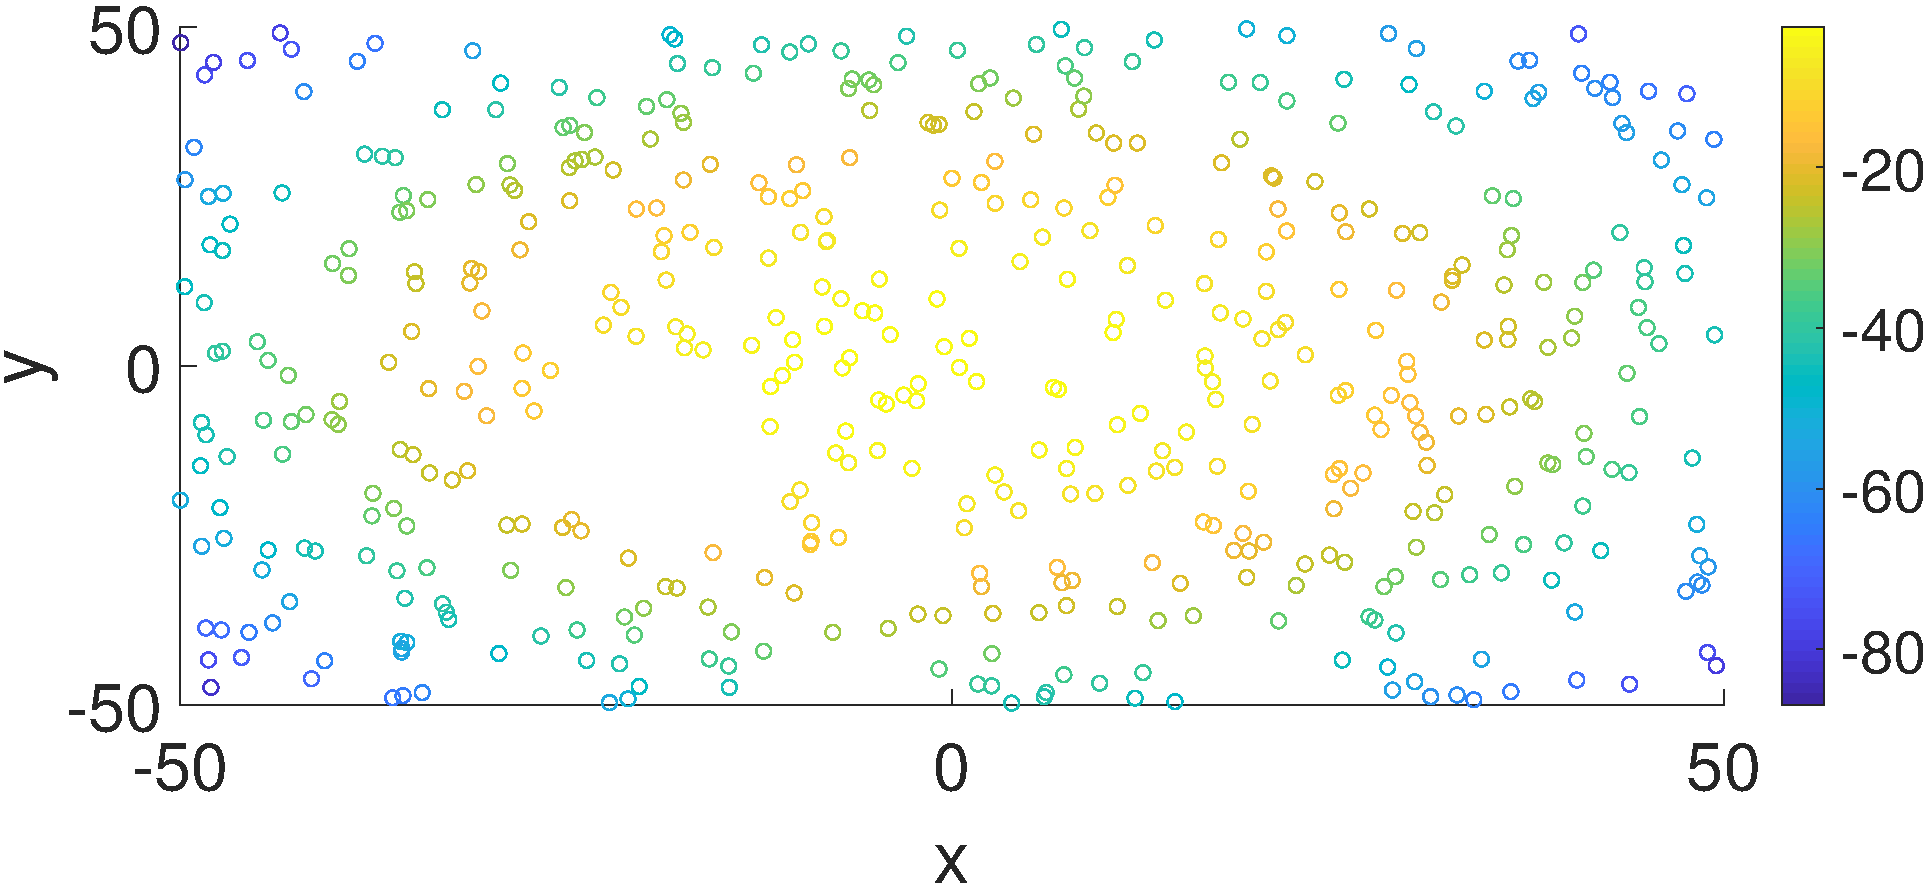
\includegraphics[width=0.45\textwidth]{Figures/LApf_particles_single_time}}
\end{subfigure}
\begin{subfigure}[Weight discrepancy with respect to $m$ averaged over 200 random trials]
{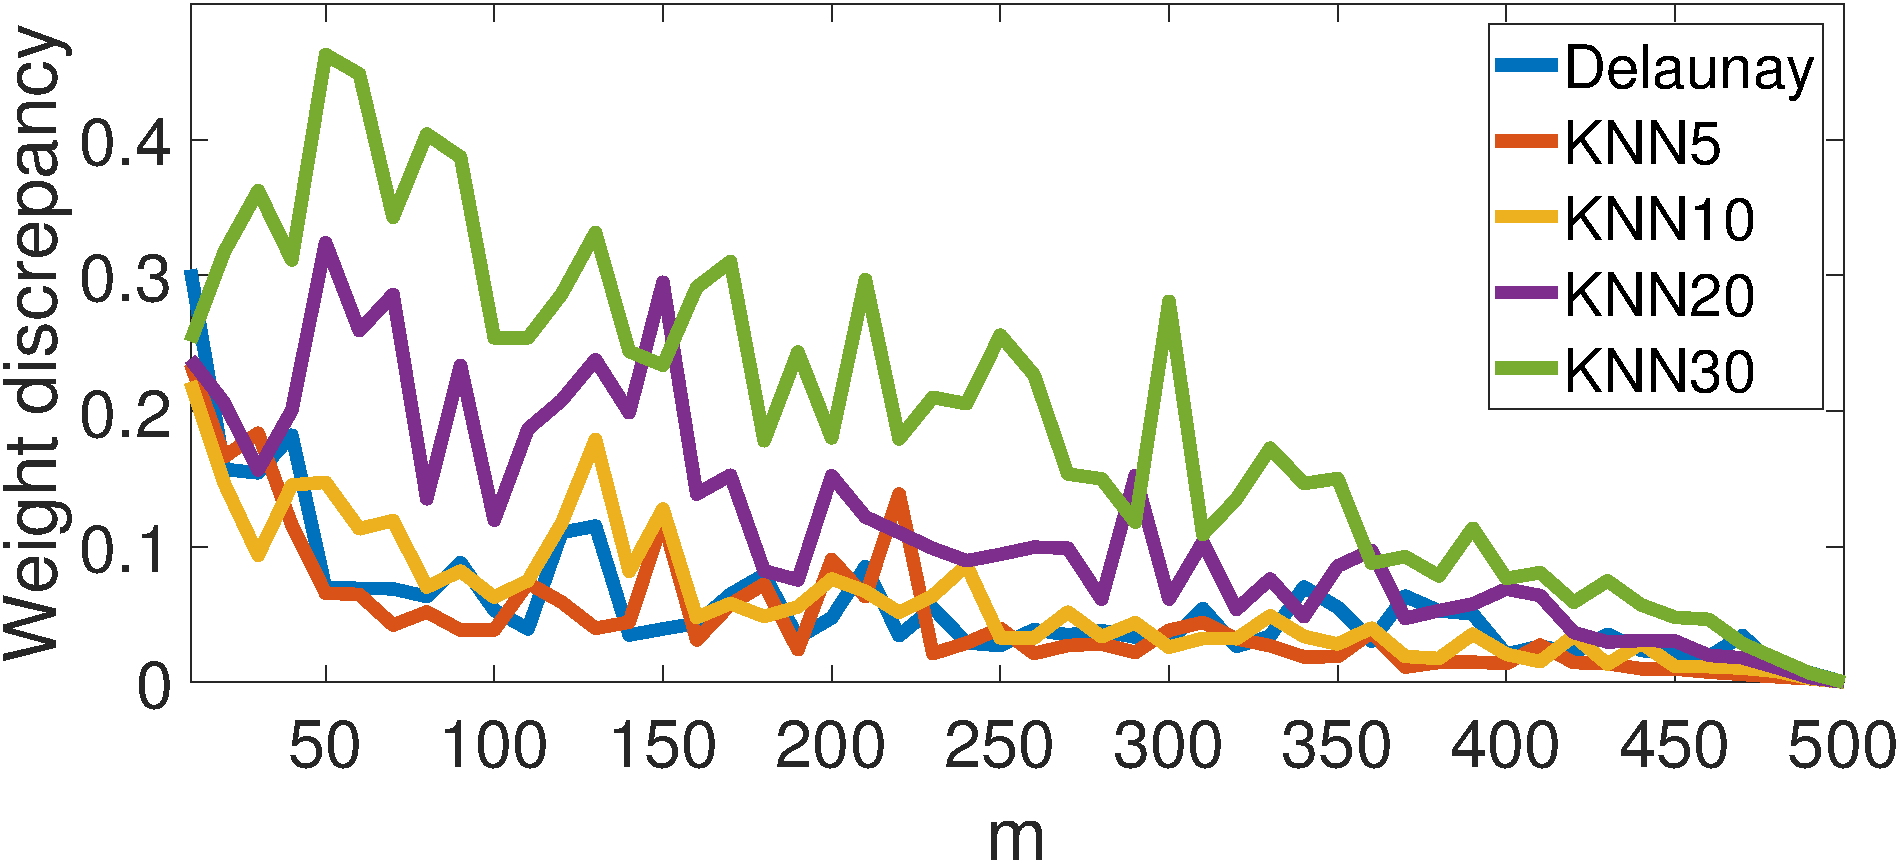
\includegraphics[width=0.45\textwidth]{Figures/LApf_single_time}}
\end{subfigure}
\caption{Weight discrepancy of LApf with respect to $m$ and different graph construction methods}
\label{fig:LApf_single_time}
\end{figure}

\section{Cluster particle filter}
A key challenge of the Laplacian particle filter is the computational burden of the eigenvalue decomposition. The \textit{Cluster particle filter} (CLusterpf) seeks to exploit the graph Laplacian while avoiding the computational burden of LApf. 

In Clusterpf, the particles are grouped into $K$ clusters based on their position. Let $C$ denote the $K \times N$ cluster assignment matrix where $C(i,j)=1$ if particle $j$ belongs to cluster $i$. The log-likelihood of the $i^{th}$ cluster, $\gamma_c^i$, is equal to the aggregate log-likelihoods of its constituent particles. We can thus relate the cluster log-likelihoods to the particle log-likelihoods as follows:
\begin{equation}
\gamma_c = C\gamma
\end{equation}

Rather than gossiping on the $N\times 1$ vector $\gamma^s$, each sensor only needs to broadcast the $K\times 1$ vector $\gamma_c$. When $K \ll N$, significant reduction in communication overhead can achieved. After reaching consensus on $\gamma_c$, we need to recover the individual particle joint log-likelihoods. A naive solution is to simply assign equal weight to all particles in a cluster; but this leads to poor results as the resulting log-likelihoods exhibit sharp change at cluster boundary. Instead, we exploit the graph Laplacian to ensure that the log-likelihood values remain smooth over the state space. We again construct a Delaunay triangulation graph over the particles, compute the Laplacian matrix $L$, and then solve the following convex minimization problem:
\begin{align}
\underset{\gamma}{\text{minimize}}& \quad \gamma^TL\gamma  \\
\text{subject to}& \quad C\gamma = \gamma_c
\end{align}
In other words, we seek to assign particle log-likelihood values that are smooth with respect to particle proximity while ensuring the aggregate values are equal to the cluster value. Since the matrix $L$ is positive semi-definite, the problem is convex, has a global minimum and can be solved using well-known methods~\cite{Boyd2004}.

We now derive the computational overhead of the cluster filter. K-mean clustering has complexity $O(4NKI)$~\cite{Hartigan1979} where $I$ is the number of clustering iterations and the constant $4$ is the target state dimension. $K$ cluster log-likelihoods are then aggregated across all sensors. We again have Delaunay triangulation for graph construction. The log-likelihood is recovered via convex minimization with complexity $O(\sqrt{N})$~\cite{Potra2000}. The overall complexity is thus $O(SNKI+SKNGossip + SN+S\sqrt{N})\subset O(SNKI)$. For $K\ll N$ and $I \ll N$, Clusterpf has a significantly lower computational overhead than LApf. 

Fig.~\ref{fig:Clusterpf_single_time} shows the average weight discrepancy of Clusterpf with respect to $K$. At low $K$, the Delaunay triangulation graph offers competitive performance without the need of tuning an additional parameter. For the remainder of the paper, we consider only Delaunay triangulation for graph construction in Clusterpf. 

\begin{figure}
\centering
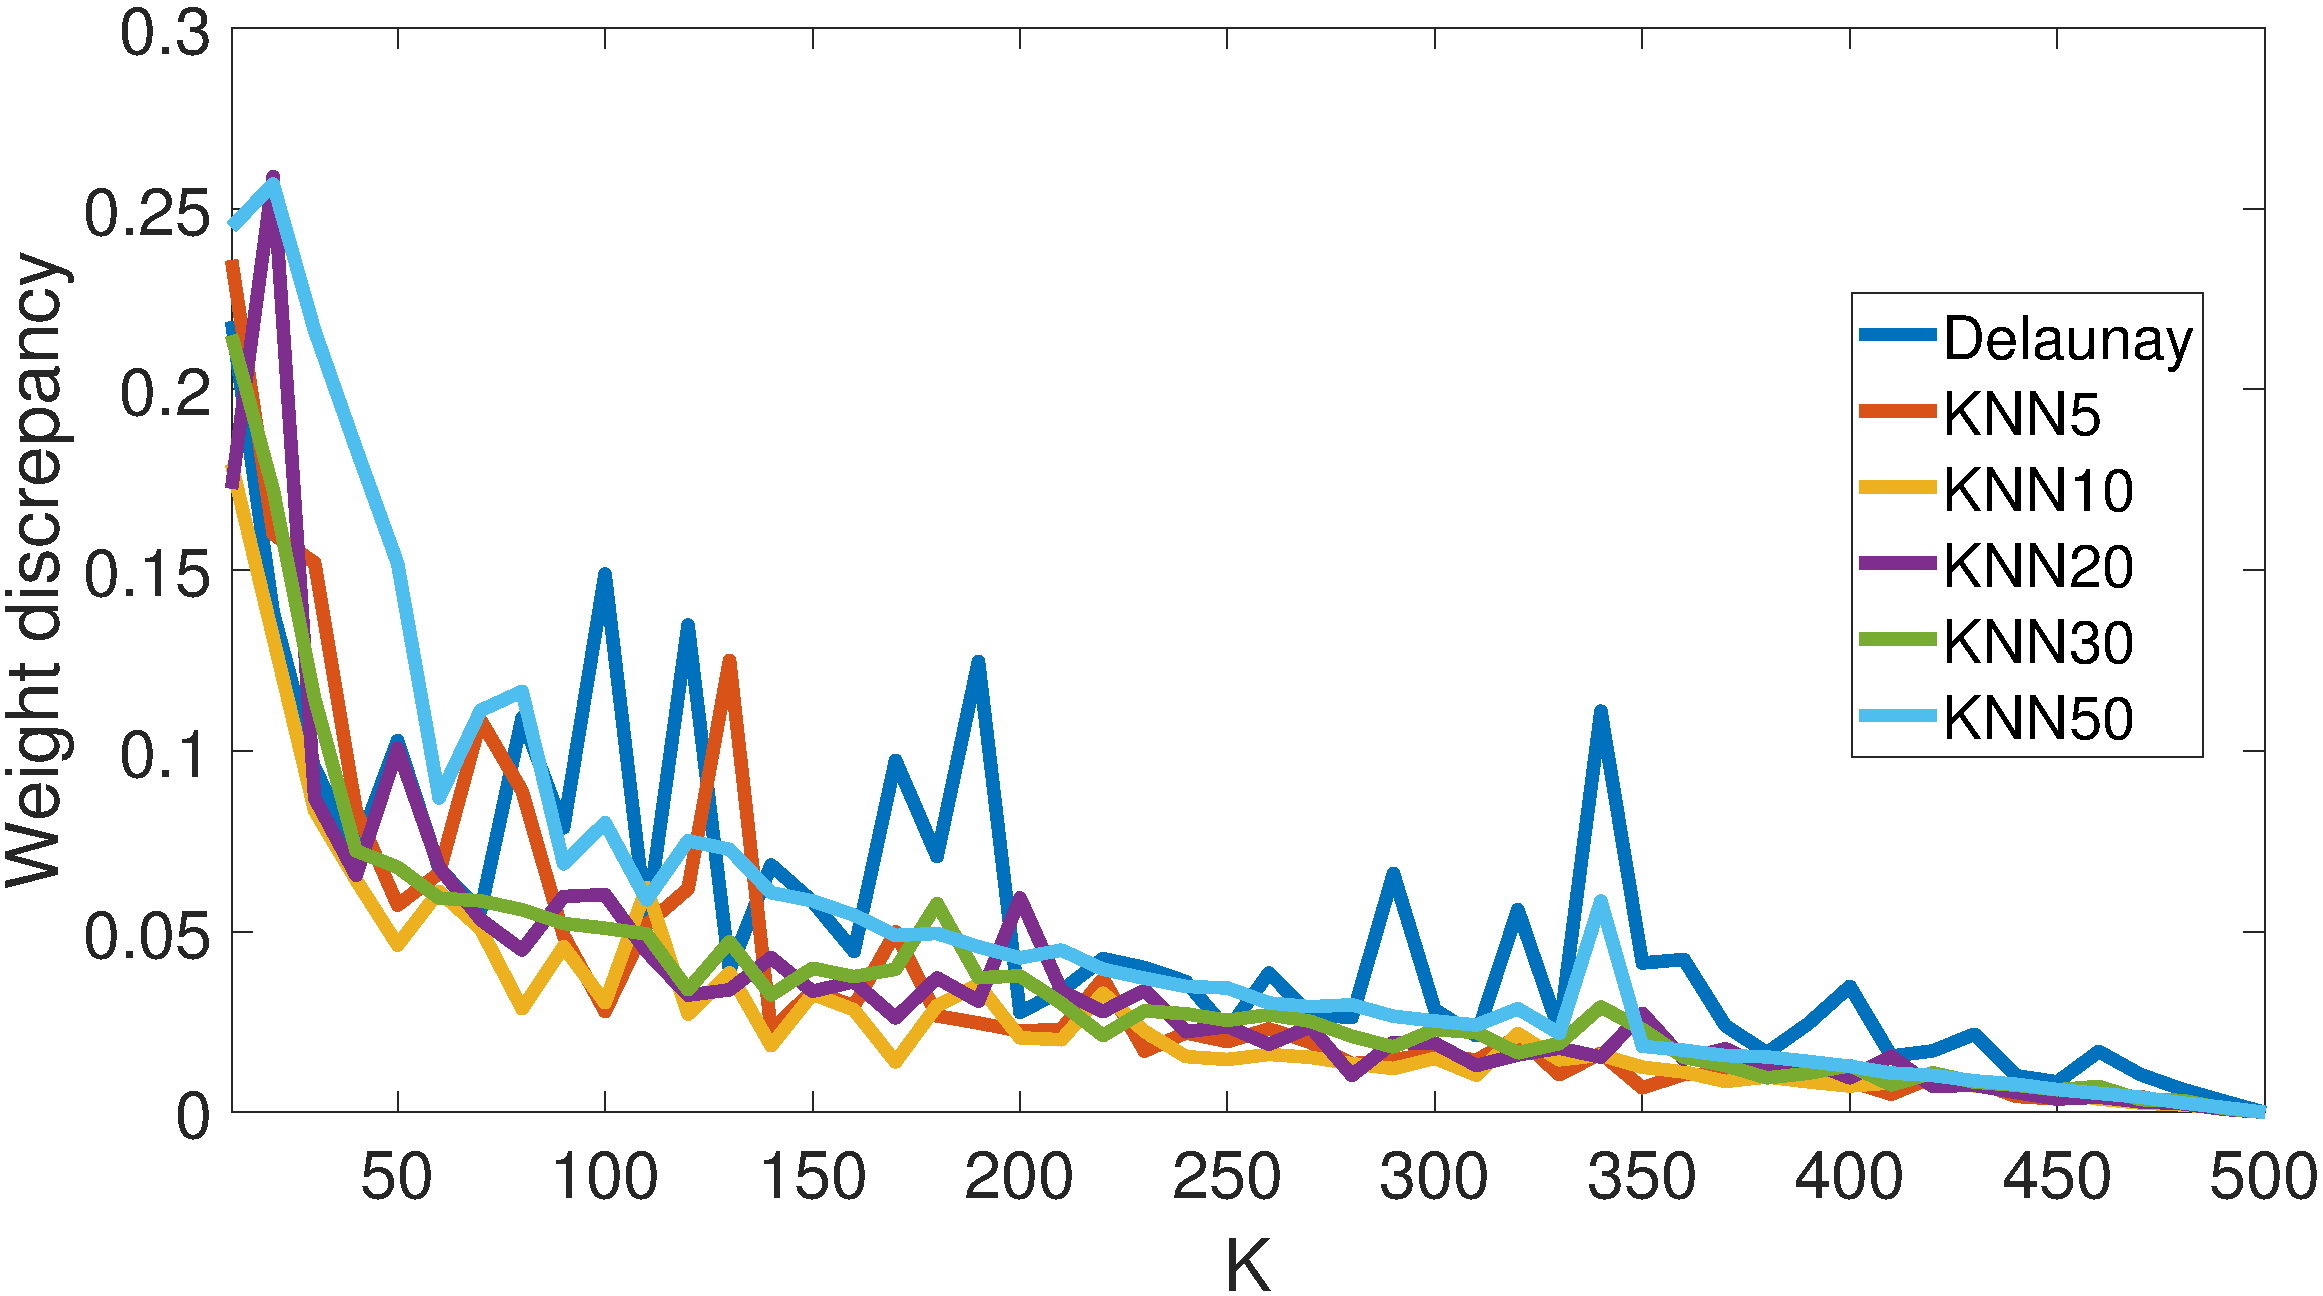
\includegraphics[width=0.45\textwidth]{Figures/Clusterpf_single_time}
\caption{Weight discrepancy with respect to $K$ averaged over 200 trials}
\label{fig:Clusterpf_single_time}
\end{figure}

\section{Numerical study}
\label{sec:evaluation}
In this section, we evaluate the performance of the two presented filters. For comparison, we also include the \textit{likelihood consensus particle filter} (LCpf)~\cite{Hlinka2012}, \textit{constraint sufficient statistics particle filter} (CSSpf)~\cite{Mohammadi2014} and a centralized bootstrap particle filter as baseline. We consider two different simulated tracks with different measurement models. Each track contains a network of $S$ static sensors which collaboratively track a moving target over 50 time steps. Fig.~\ref{fig:test_tracks} shows the two test tracks.

\begin{figure}[h]
\centering
\begin{subfigure}[Track 1]
{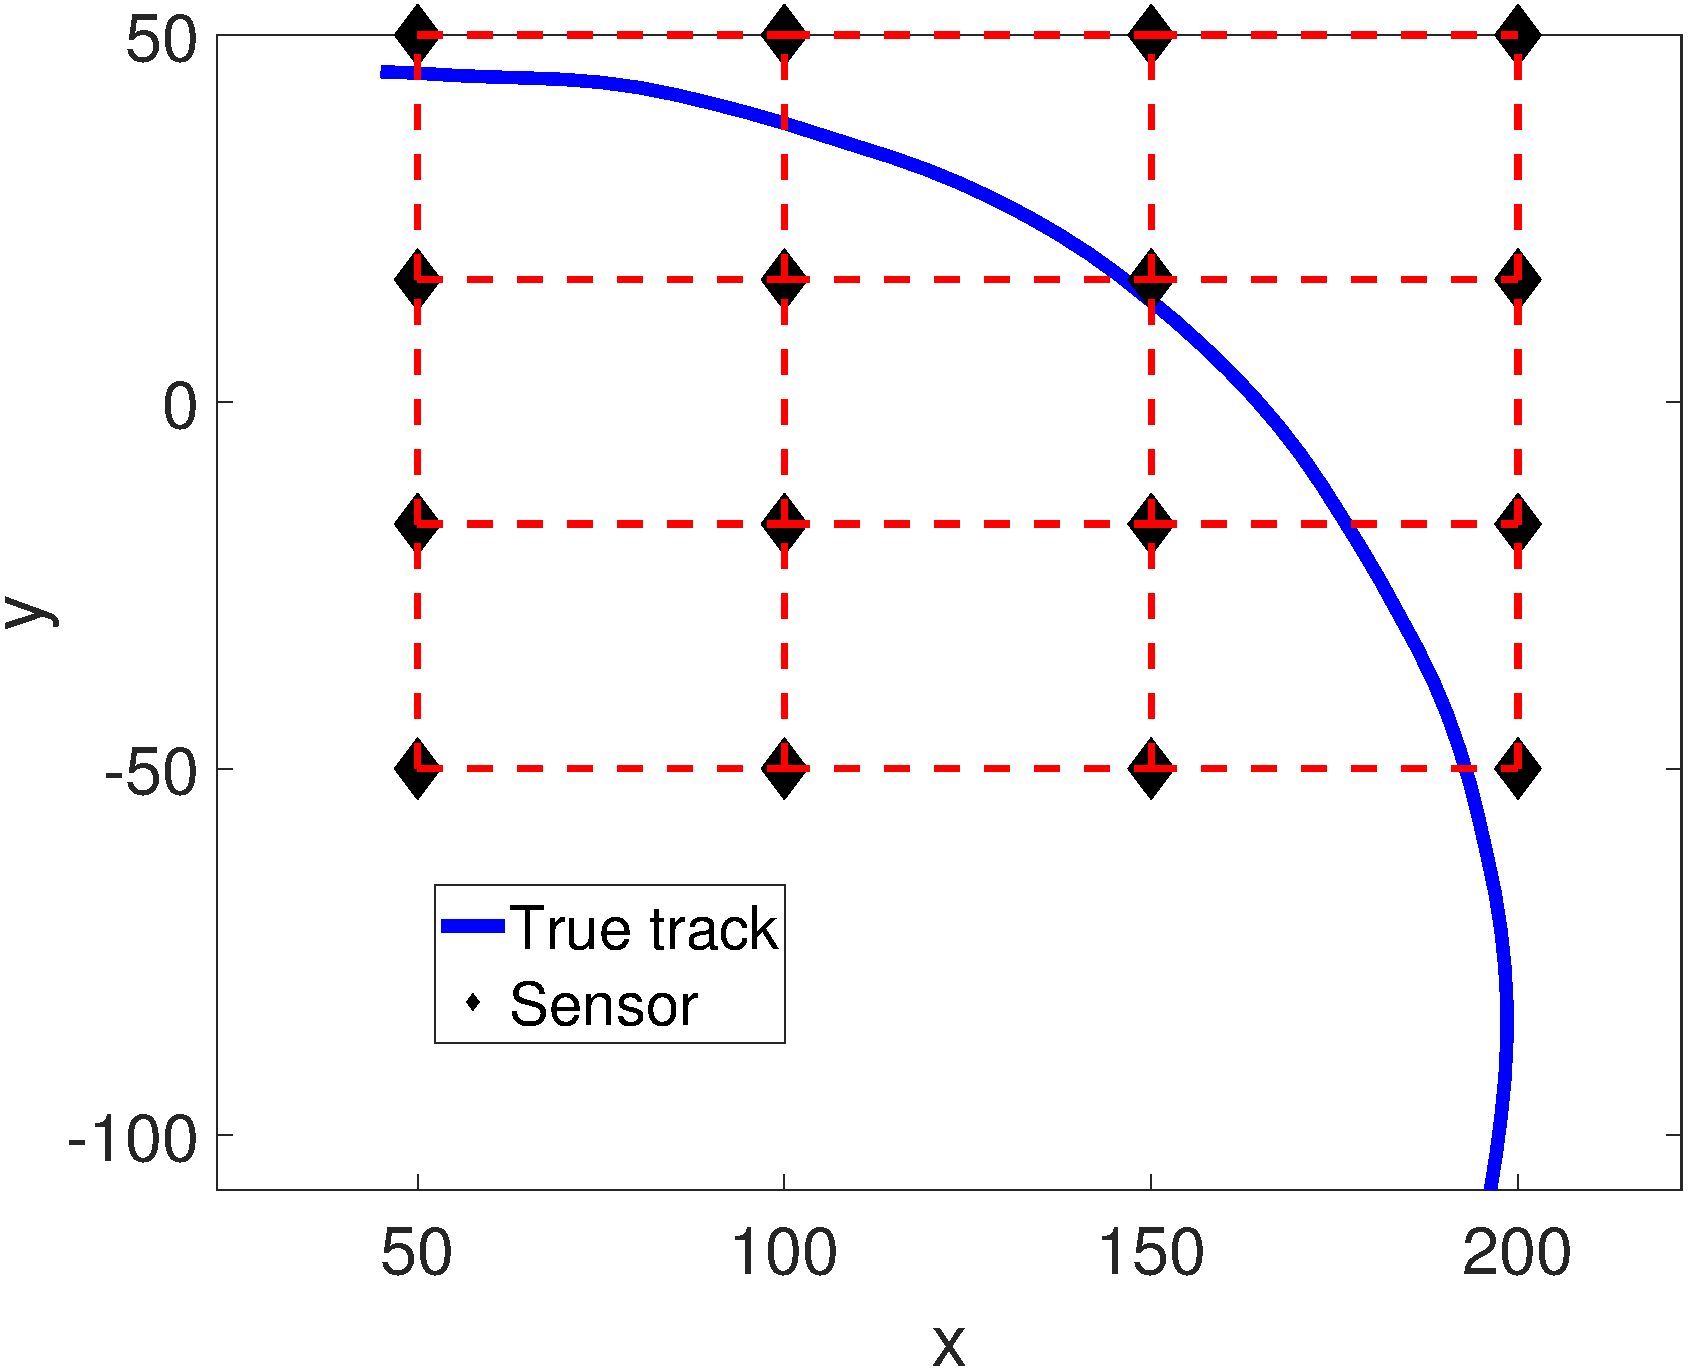
\includegraphics[width=0.4\textwidth]{Figures/Track1}}
\end{subfigure}
\begin{subfigure}[Track 2]
{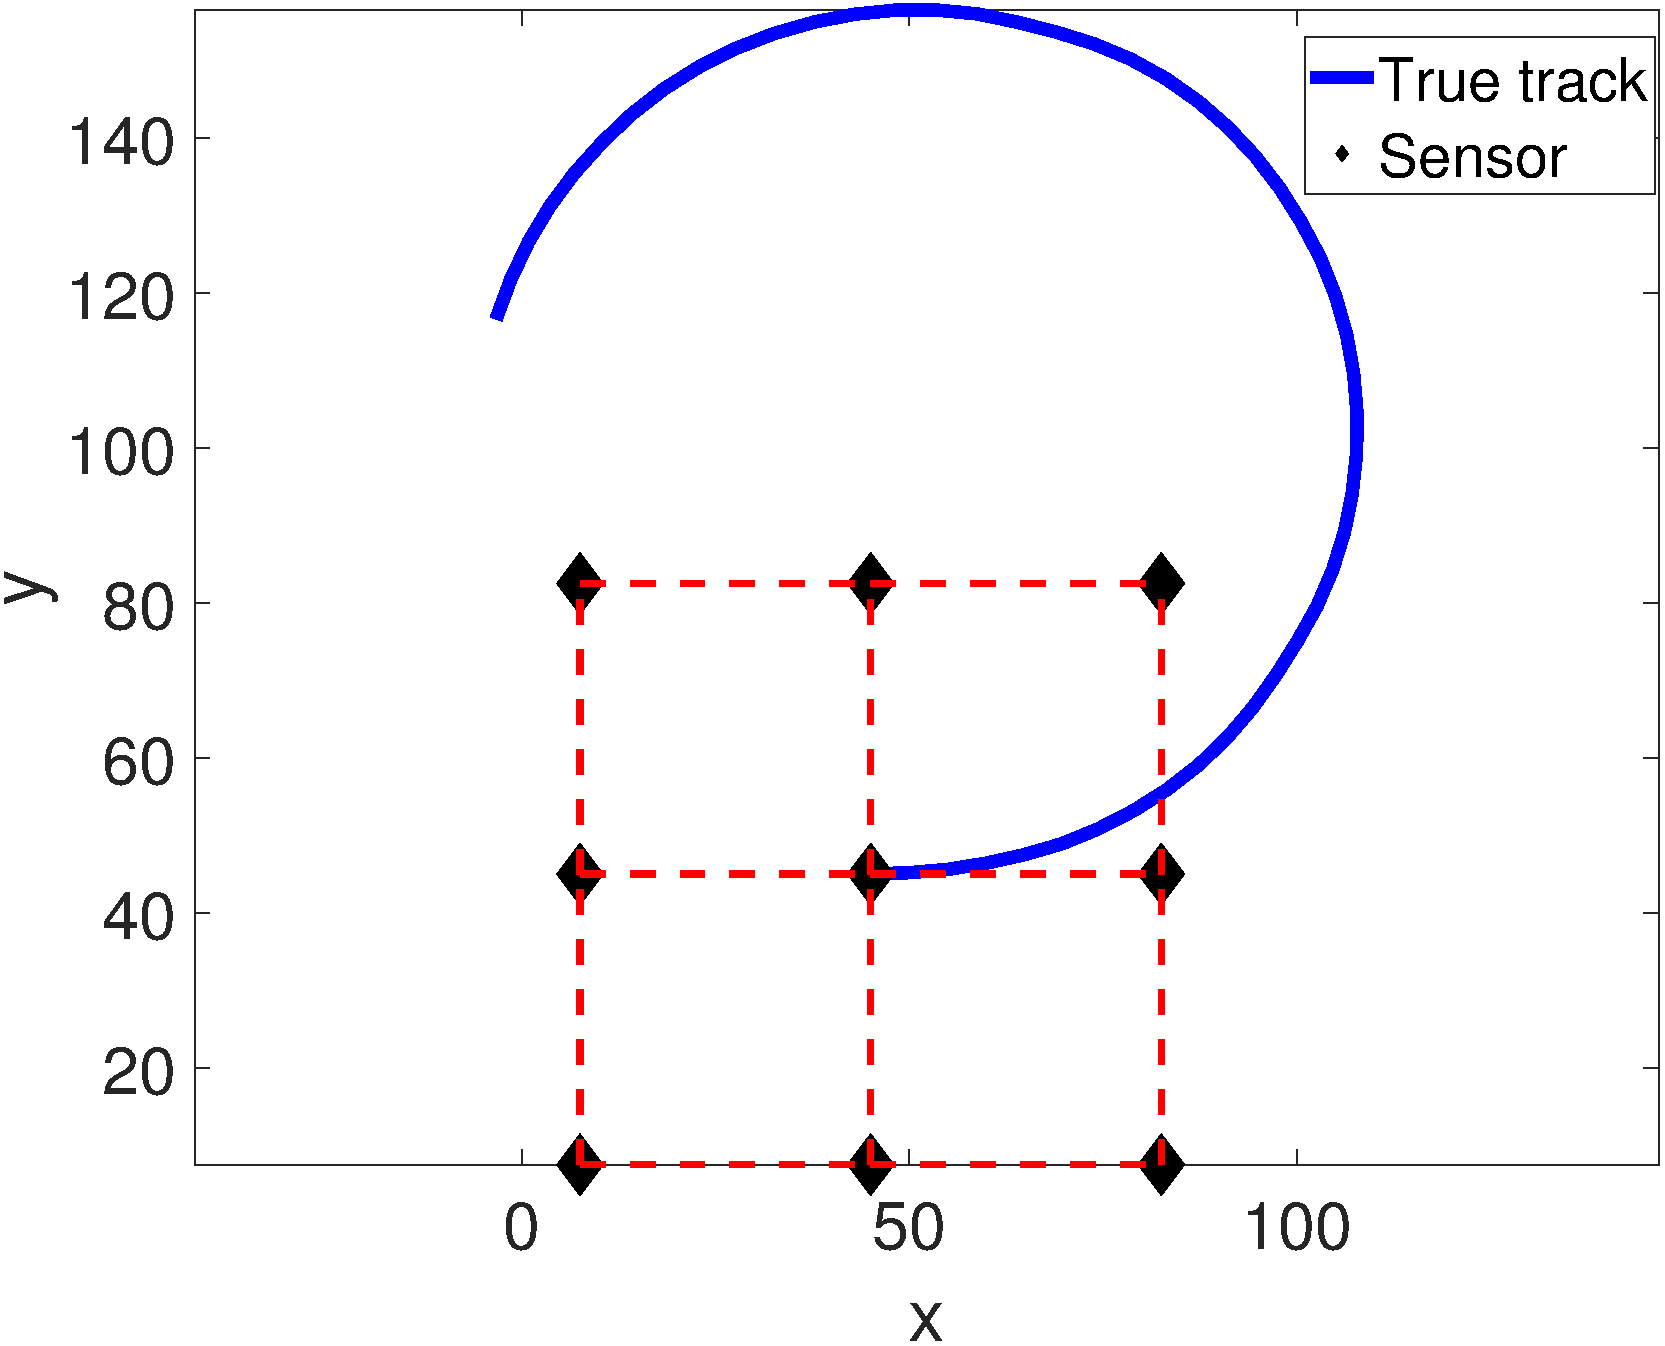
\includegraphics[width=0.4\textwidth]{Figures/Track2}}
\end{subfigure}
\caption{Target tracks (blue curve) and sensor positions (black diamond). Sensors connected by red dashed lines are within broadcast range of each other.}
\label{fig:test_tracks}
\end{figure}

The target state evolves over time following a discrete-time model:
\begin{equation}
X(k+1) = F(X(k))+\xi(k)
\end{equation}
where $F(X(k))$ is the dynamic model and $\xi(k)$ is the zero-mean Gaussian process noise. The simulated target randomly switches between two different motion models: constant velocity with probability $P_{cv} = 0.05$ and coordinated turn with probability $1-P_{cv}=0.95$. 

For constant velocity, we have
\begin{equation}
F(X(k)) = 
\left[
\begin{array}{cccc}
1 & 0 & 1 & 0 \\
0 & 1 & 0 & 1 \\
0 & 0 & 1 & 0 \\
0 & 0 & 0 & 1
\end{array}
\right]
\end{equation}

For coordinated turn, we have 
\begin{equation}
F(X(k)) = 
\left[
\begin{array}{cccc}
1 & 0 & \frac{\sin(\Omega)}{\Omega (k)} & -\frac{1-\cos(\Omega (k))}{\Omega (k)} \\
0 & 1 & \frac{1-\cos(\Omega (k))}{\Omega (k)} & \frac{\sin(\Omega (k))}{\Omega (k)} \\
0 & 0 & \cos(\Omega (k)) & -\sin(\Omega (k)) \\
0 & 0 & \sin(\Omega (k)) & \cos(\Omega (k)) 
\end{array}
\right]
\end{equation}
where $\Omega (k)$ is the turning rate
\begin{equation}
\Omega (k) = \frac{a}{\sqrt{\dot{x}^2(k)+\dot{y}^2(k)}}
\end{equation}
with $a=0.5$ being the maneuver acceleration parameter. 

In the first simulated track, all sensors receive noisy bearing measurements (in radians) from the target.
\begin{equation}
H_s(X(k))= \arctan2 \left( \frac{x_t(k)-x_s}{y_t(k)-y_s} \right) + \eta(k)
\end{equation}
where $\eta(k)$ is the zero-mean Gaussian measurement noise. In the second track, the sensors receive noisy range measurements (in km).
\begin{equation}
H_s(X(k)) = \sqrt{(x_t(k)-x_s)^2+(y_t(k)-y_s)^2} + \eta(k)
\end{equation}

The process and measurement noises $\xi(k)$ and $\eta(k)$ have covariance matrices $Q$ and $R$ respectively.
\begin{align}
Q &= \sigma_a^2
\left[
\begin{array}{cccc}
\frac{1}{3} & 0 & \frac{1}{2} & 0 \\
0 & \frac{1}{3} & 0 & \frac{1}{2} \\
\frac{1}{2} & 0 & 1 & 0 \\
0 & \frac{1}{2} & 0 & 1 \\
\end{array}
\right]\\
R_{\text{bearing}} &= \sigma_{\theta}^2 \\
R_{\text{range}} &= \sigma_{r}^2
\end{align}
where $\sigma_a=10^{-4}$, $\sigma_{\theta}=0.0873\text{ rad} = 5 \text{ degree}$, and $\sigma_{r}= 5 \text{ km}$.

%\begin{figure}
%\centering
%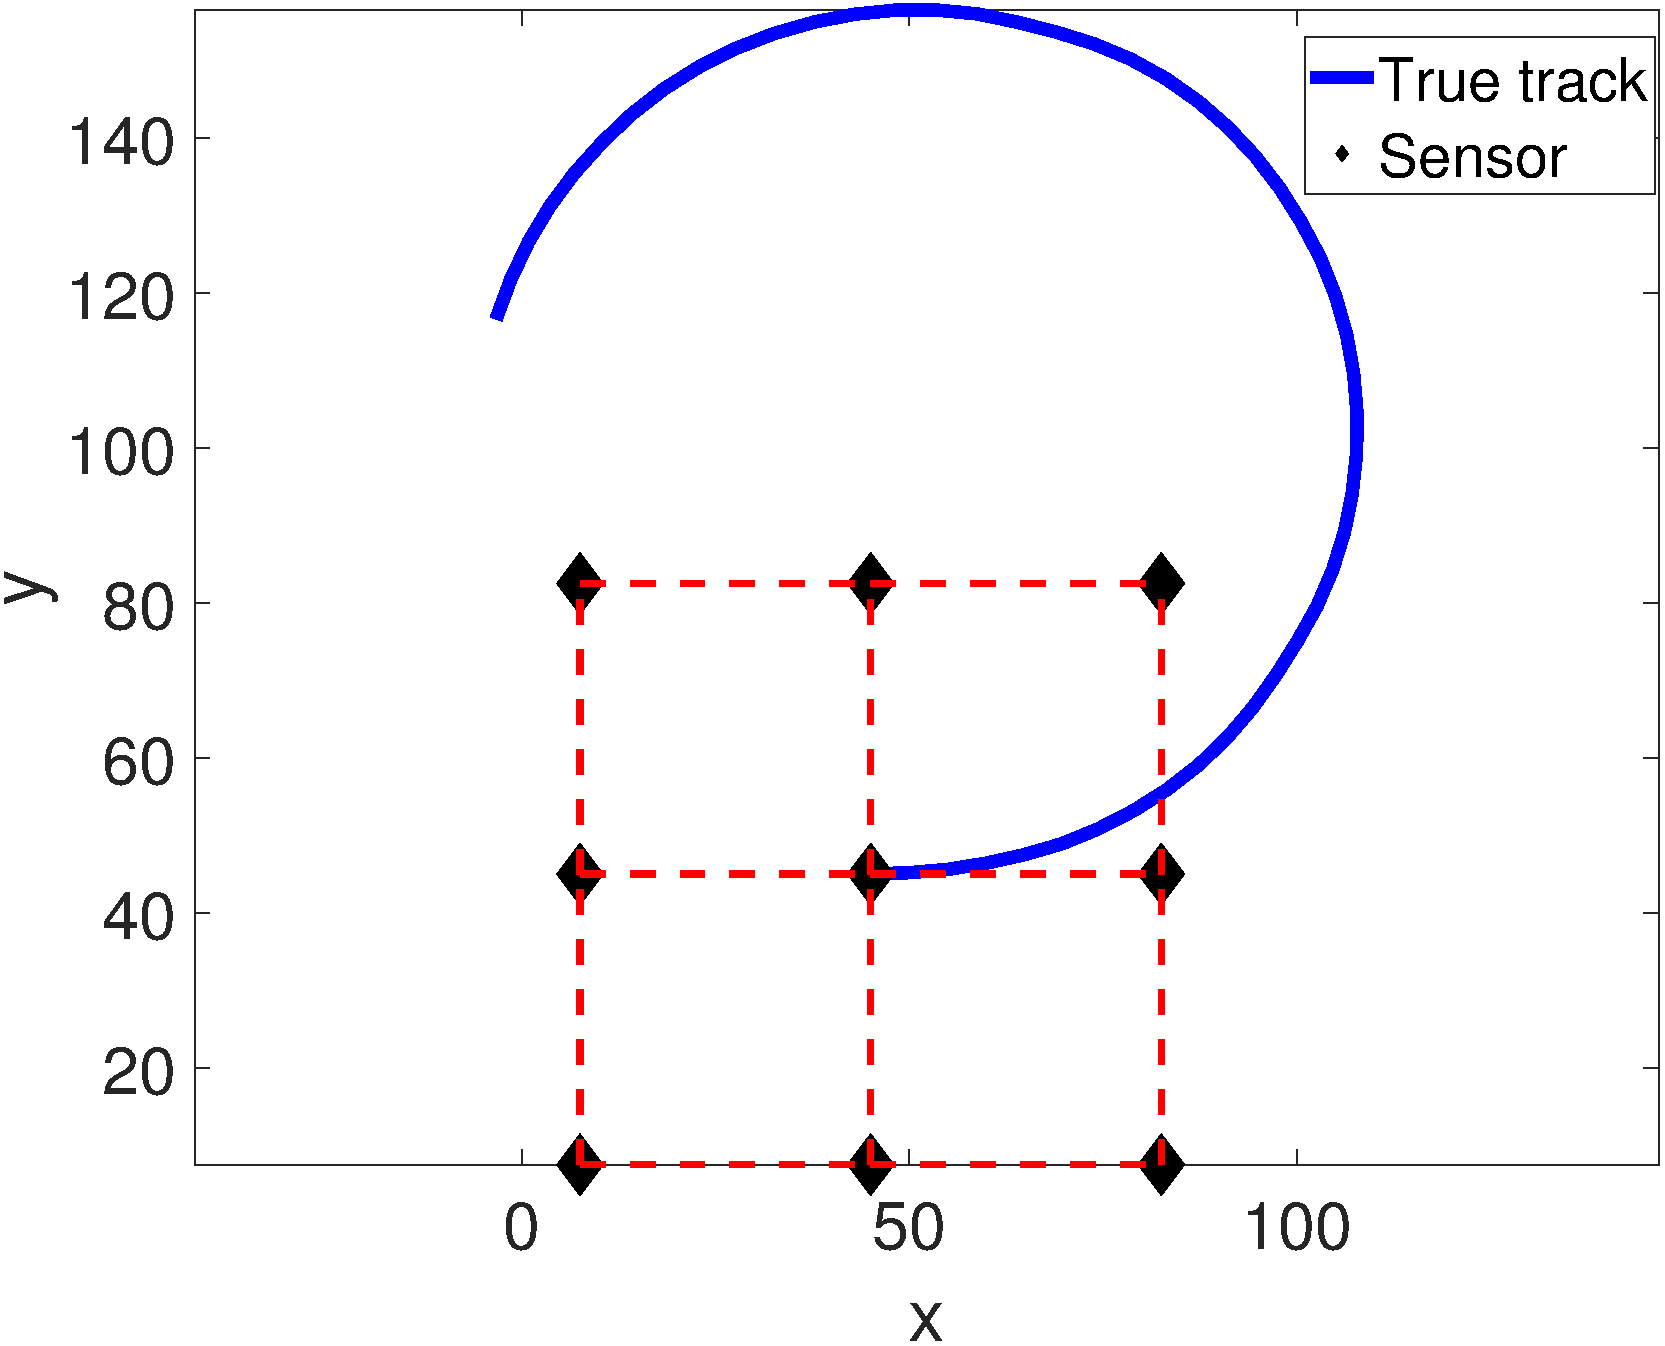
\includegraphics[width=0.45\textwidth]{Figures/track}
%\caption{Target trajectory (blue curve) and sensor positions (black diamond). Sensors connected by red dashed lines are within broadcast range of each other.}
%\label{fig:track}
%\end{figure}

All particle filters use a total of $N=500$ particles. At time step 1, we generate the initial particles using the true target state: $X_i(1) \sim \mathcal{N}(X(1), R_{\text{initial}})$ with $R_{\text{initial}}=\text{diag}([0.5^2,0.5^2,0.05^2,0.05^2])$. For LCpf, we use a set of basis functions involving all permutations of $x_t^iy_t^j$ with $0\leq i, j \leq d$ where $d$ is some user-specified max polynomial degree (i.e., For $d=2$, the basis functions would be $\beta_1(X) = x_t^0 y_t^0 = 1, \beta_2(X) = x_t^0 y_t^1 = y_t, ..., \beta_9(X) = x_t^2 y_t^2 $.). We also include a modified version of LCpf. We define the matrix $\Psi^{LC}$ where $\Psi^{LC}(i,j)=\beta_j(X_i)$. We apply Gram-Schmidt orthogonalization to $\Psi^{LC}$ so that all columns are orthogonal to each other and have unit norm. The columns of $\Psi^{LC}$ thus provide a basis for encoding log-likelihoods and have a role analogous to the eigenvectors in LApf. This filter is henceforth referred to as LCpf-GS and the reason for its inclusion will be explained in the next section. For LApf, we construct a Delaunay triangulation graph and retain $m<N$ eigenvectors as the basis of Laplacian transformation. Finally, for Clusterpf, all particles are grouped into $K$ clusters and a Delaunay triangulation graph is constructed to recover individual particle weights. Unless otherwise specified, we set $d=2$ so LCpf has 9 basis functions, and we set $m=K=6$. These values are chosen to match CSSpf which only uses 6 coefficients to encode the log-likelihoods and to minimize the communication overhead per sensor per gossip iteration. 

The random number generators are synchronized to ensure that the particles remain the same across sensors. Distributed summation is performed using gossip algorithms. At each time step, we perform $NGossip$ gossip iterations. At each gossip iteration, each sensor $i$ broadcasts its local values $G_i$, receives broadcasts from its neighbors, and then updates its local values as a weighted aggregate:
\begin{align}
G_{i,\text{new}} &= w_{ii}G_{i,\text{old}} + \sum_{j\in N_i}w_{ij}G_{j,\text{old}} \\
w_{ij} &=
\begin{cases}
\frac{1}{1+max(d_i, d_j)} \quad j\in N_i \\
1-\sum_{j\in N_i}w_{ij} \quad i=j \\
0 \quad j\notin N_i
\end{cases}
\label{eqn:metropolis_weight}
\end{align}
where $N_i$ denotes the set of neighboring sensors of sensor $i$, $d_i=|N_i|$, and Metropolis weight is used for the update. Since only a finite number of gossiping iterations are executed, all sensors are not guaranteed to obtain the same values. Therefore, a max-consensus algorithm is executed to ensure all sensors obtain the same values. We do not implement a loop for the gossip iterations. Instead we define an update matrix $W$ where $W(i,j)=w_{ij}$. Therefore, given initial values $G_{\text{initial}}=[G_1,...,G_S]^T$, the final values can be easily computed as 
\begin{equation}
G_{\text{final}} = W^{NGossip}G_{\text{initial}}
\end{equation}

In the remainder of the section, we run a number of Monte Carlo simulations to compare the performance of all filters. The track and the sensor positions remain the same in each trial; but the measurements differ. We evaluate the algorithms' performances using the \textit{root mean squared error} (RMSE) of position estimate and total runtime. The first metric is self-explanatory and the second metric compares the computational overhead of all filters. Note that CSSpf is not run for track 2 since it is designed for bearing-only tracking. 

Fig.~\ref{fig:simulation_results} shows the simulation results for both tracks. Consider track 1 first (left column figures). For $NGossip\leq 100$, CSSpf and LCpf break down and have very high RMSE. After crossing a threshold value (50 for CSSpf and 100 for LCpf), the RMSE drops sharply. At low $NGossip$, LApf and Clusterpf outperform the other distributed filters by a significant margin and are on-par with the centralized BSpf for $NGossip\geq 20$. More interestingly, these two filters have robust tracking performance even with just 1 gossip iteration per time step. LCpf-GS has better performance than CSSpf and LCpf but still breaks down at low $NGossip$. The LApf has the highest runtime by a significant margin due to eigenvalue decomposition as expected. The clusterpf has the second highest runtime which can be attributed to the K-means clustering and convex minimization. The LCpf-GS and CSSpf have the lowest runtime. Note that the total runtime is fairly constant over all values of $NGossip$ due to our implementation of the gossiping algorithm. 

Consider the results for track 2 (right column figures). The RMSE curves display the same trends as in track 1. The LCpf breaks down at low $NGossip$ and its RMSE drops sharply for $NGossip>10$. The LApf and Clusterpf consistently outperform the other distributed filters at low overhead. The LCpf-GS again outperforms LCpf and achieves performance on-par with LApf for $NGossip\geq 8$. The curves for total runtime exhibit the same trends as in track 1 with LApf being the slowest by far. 

\begin{figure}[h]
\centering
\begin{subfigure}[Track 1, RMSE]
{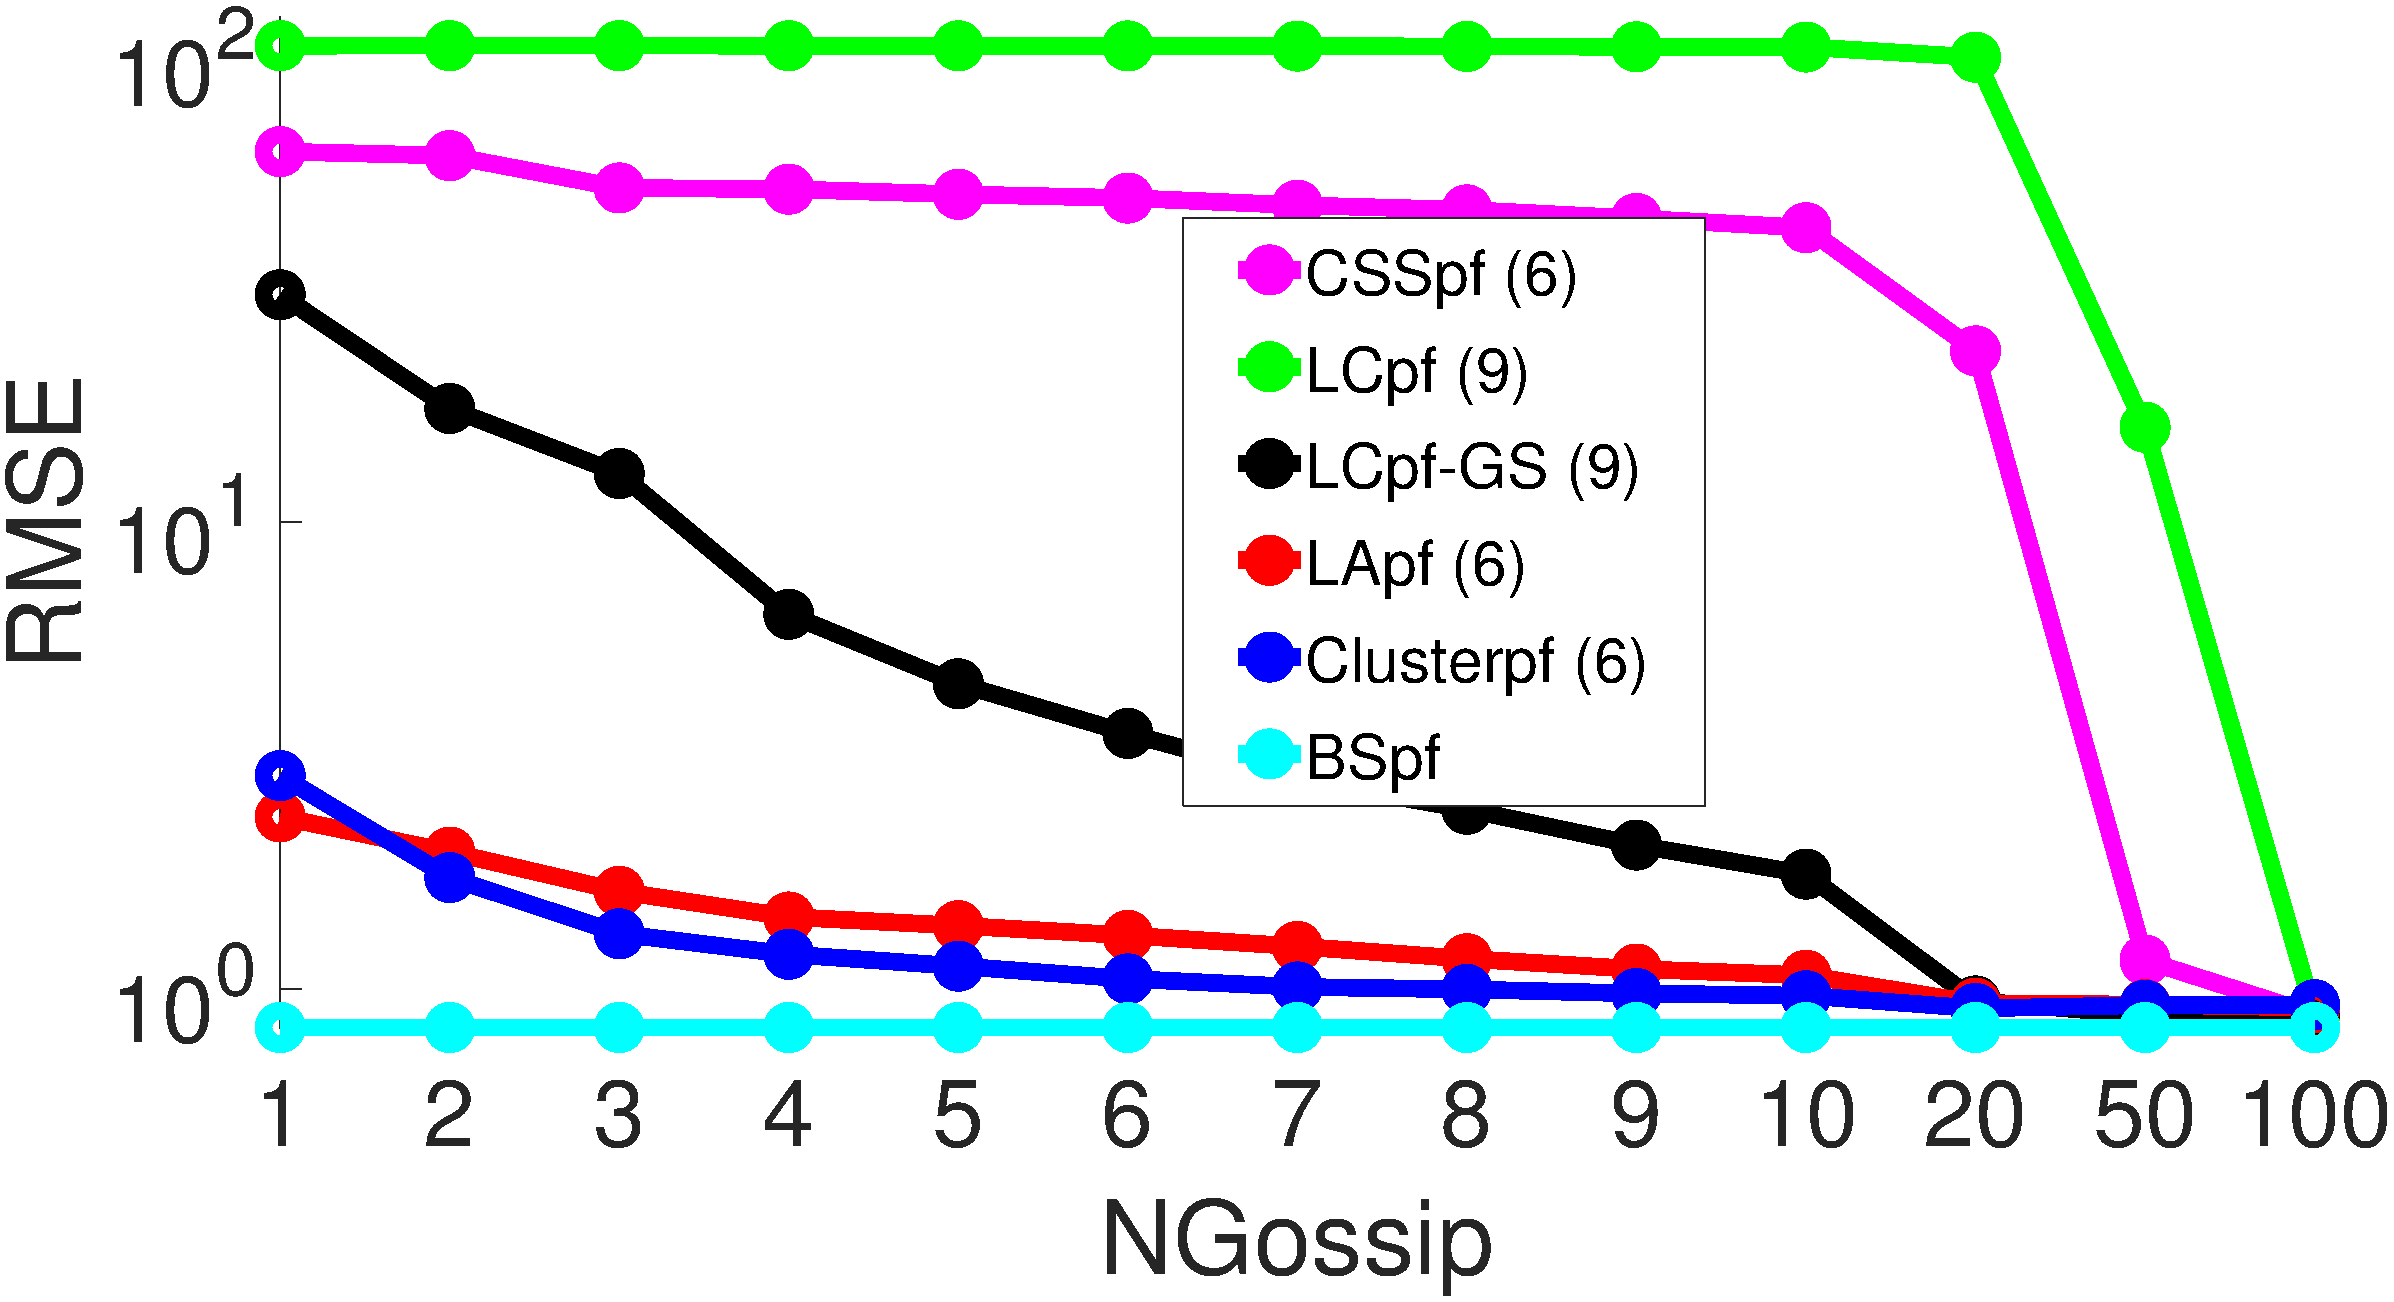
\includegraphics[width=0.45\textwidth]{Figures/Track1_RMSE_full}}
\end{subfigure}
\begin{subfigure}[Track 2, RMSE]
{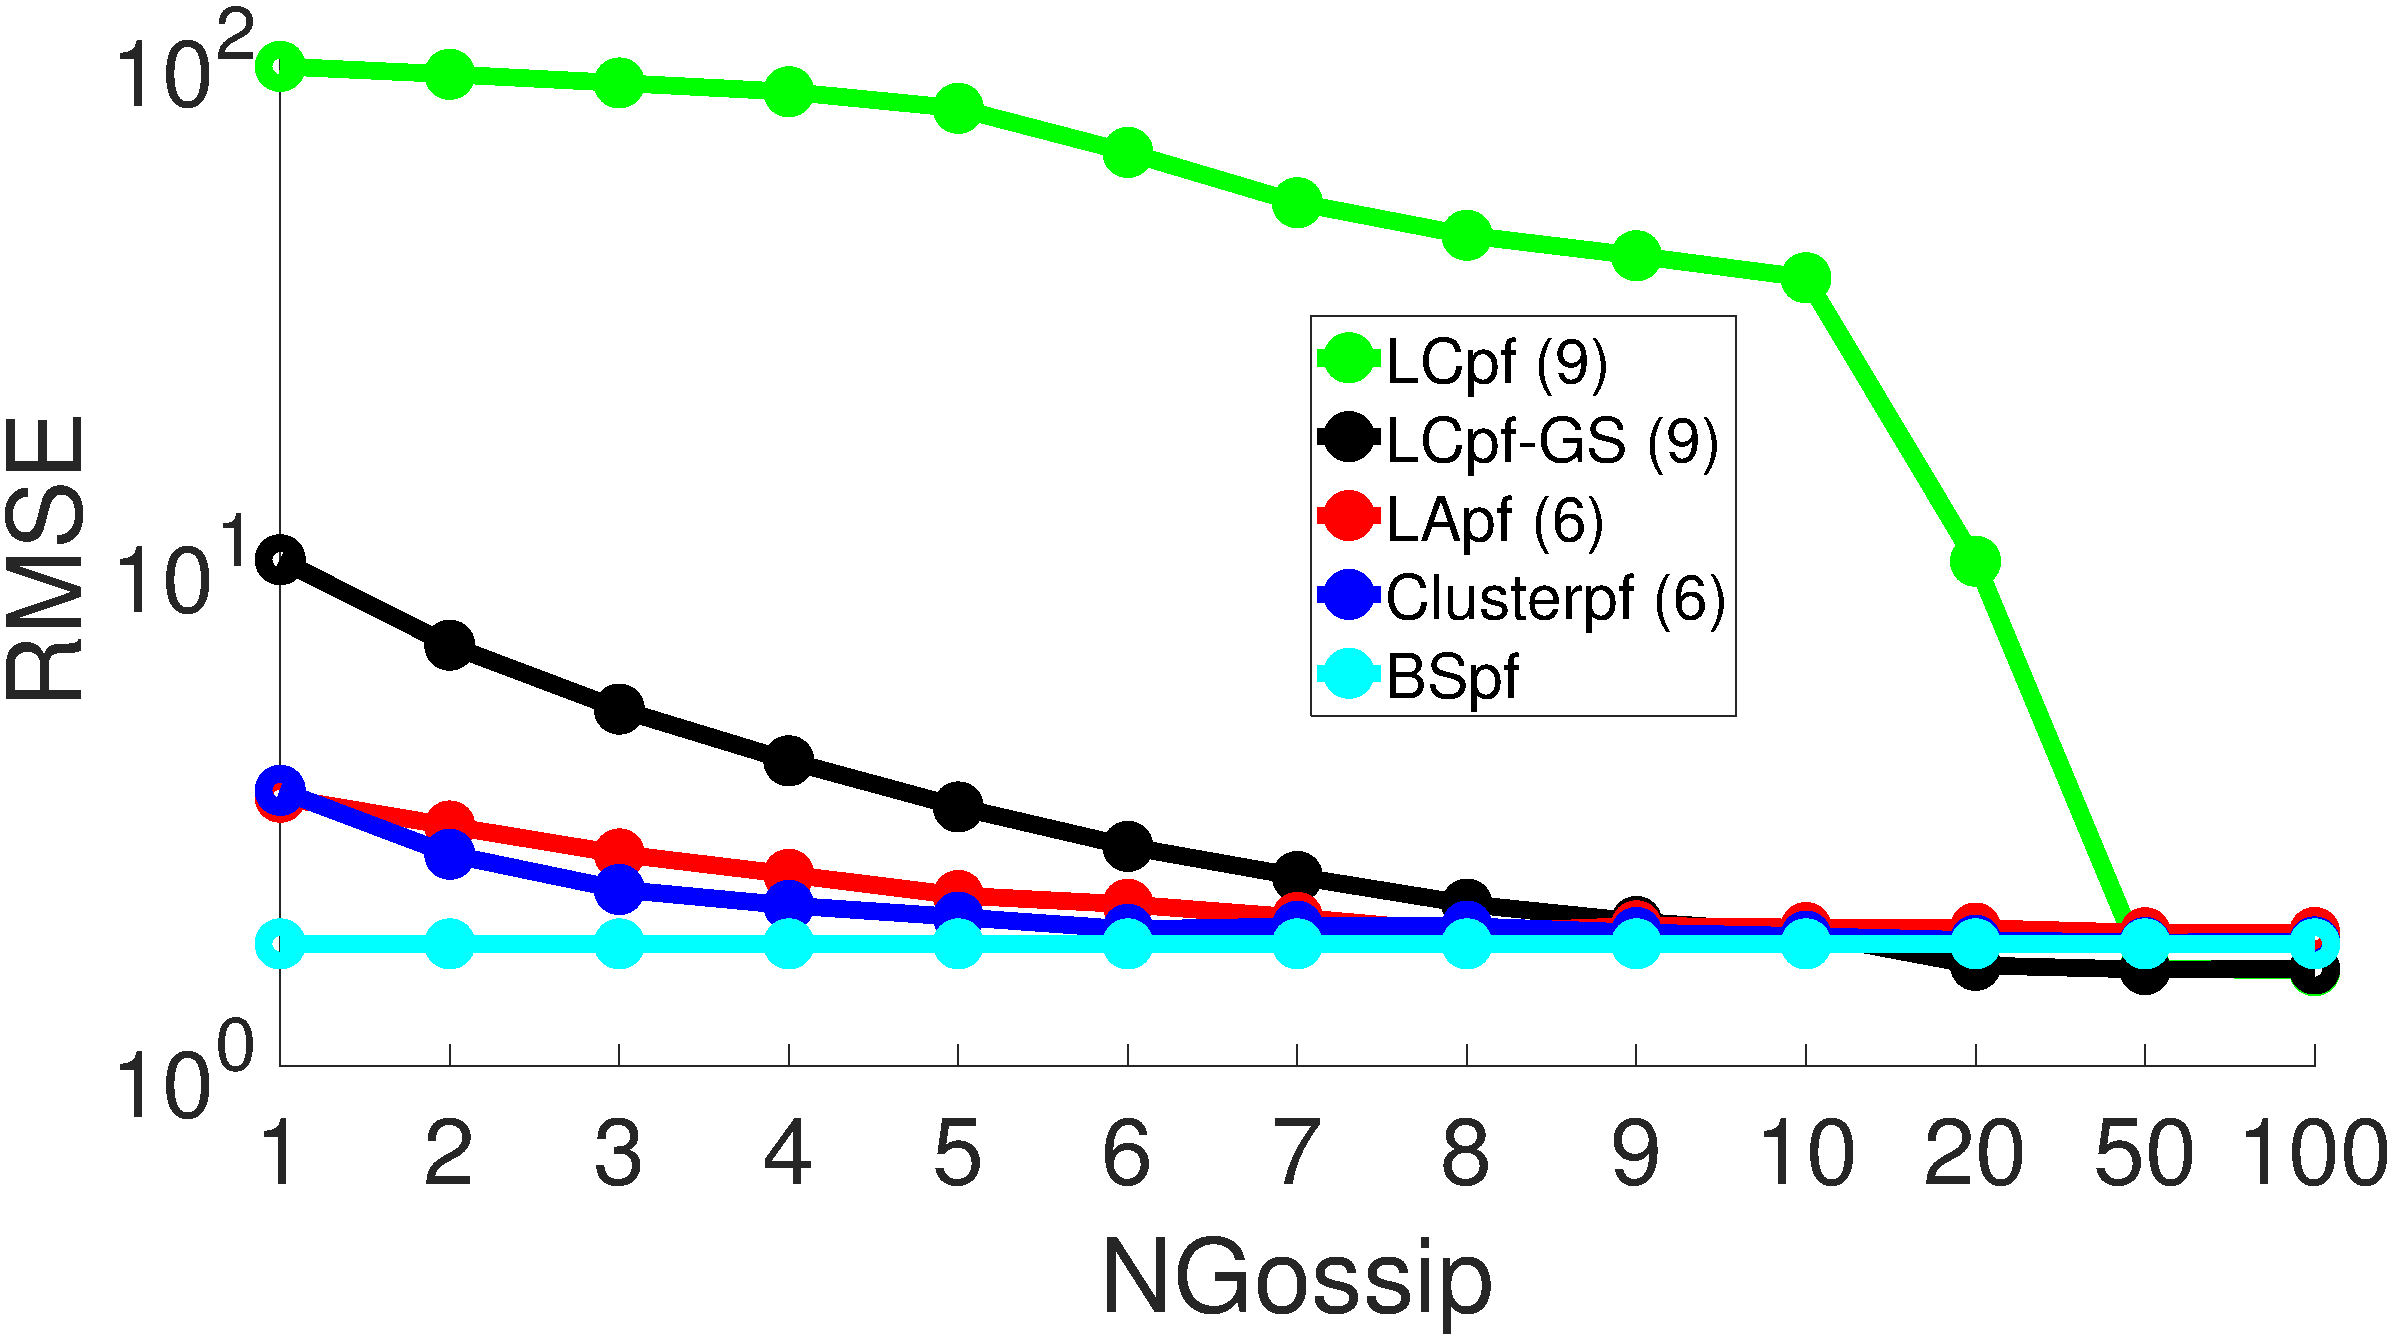
\includegraphics[width=0.45\textwidth]{Figures/Track2_RMSE_full}}
\end{subfigure}
\begin{subfigure}[Track 1, Total runtime]
{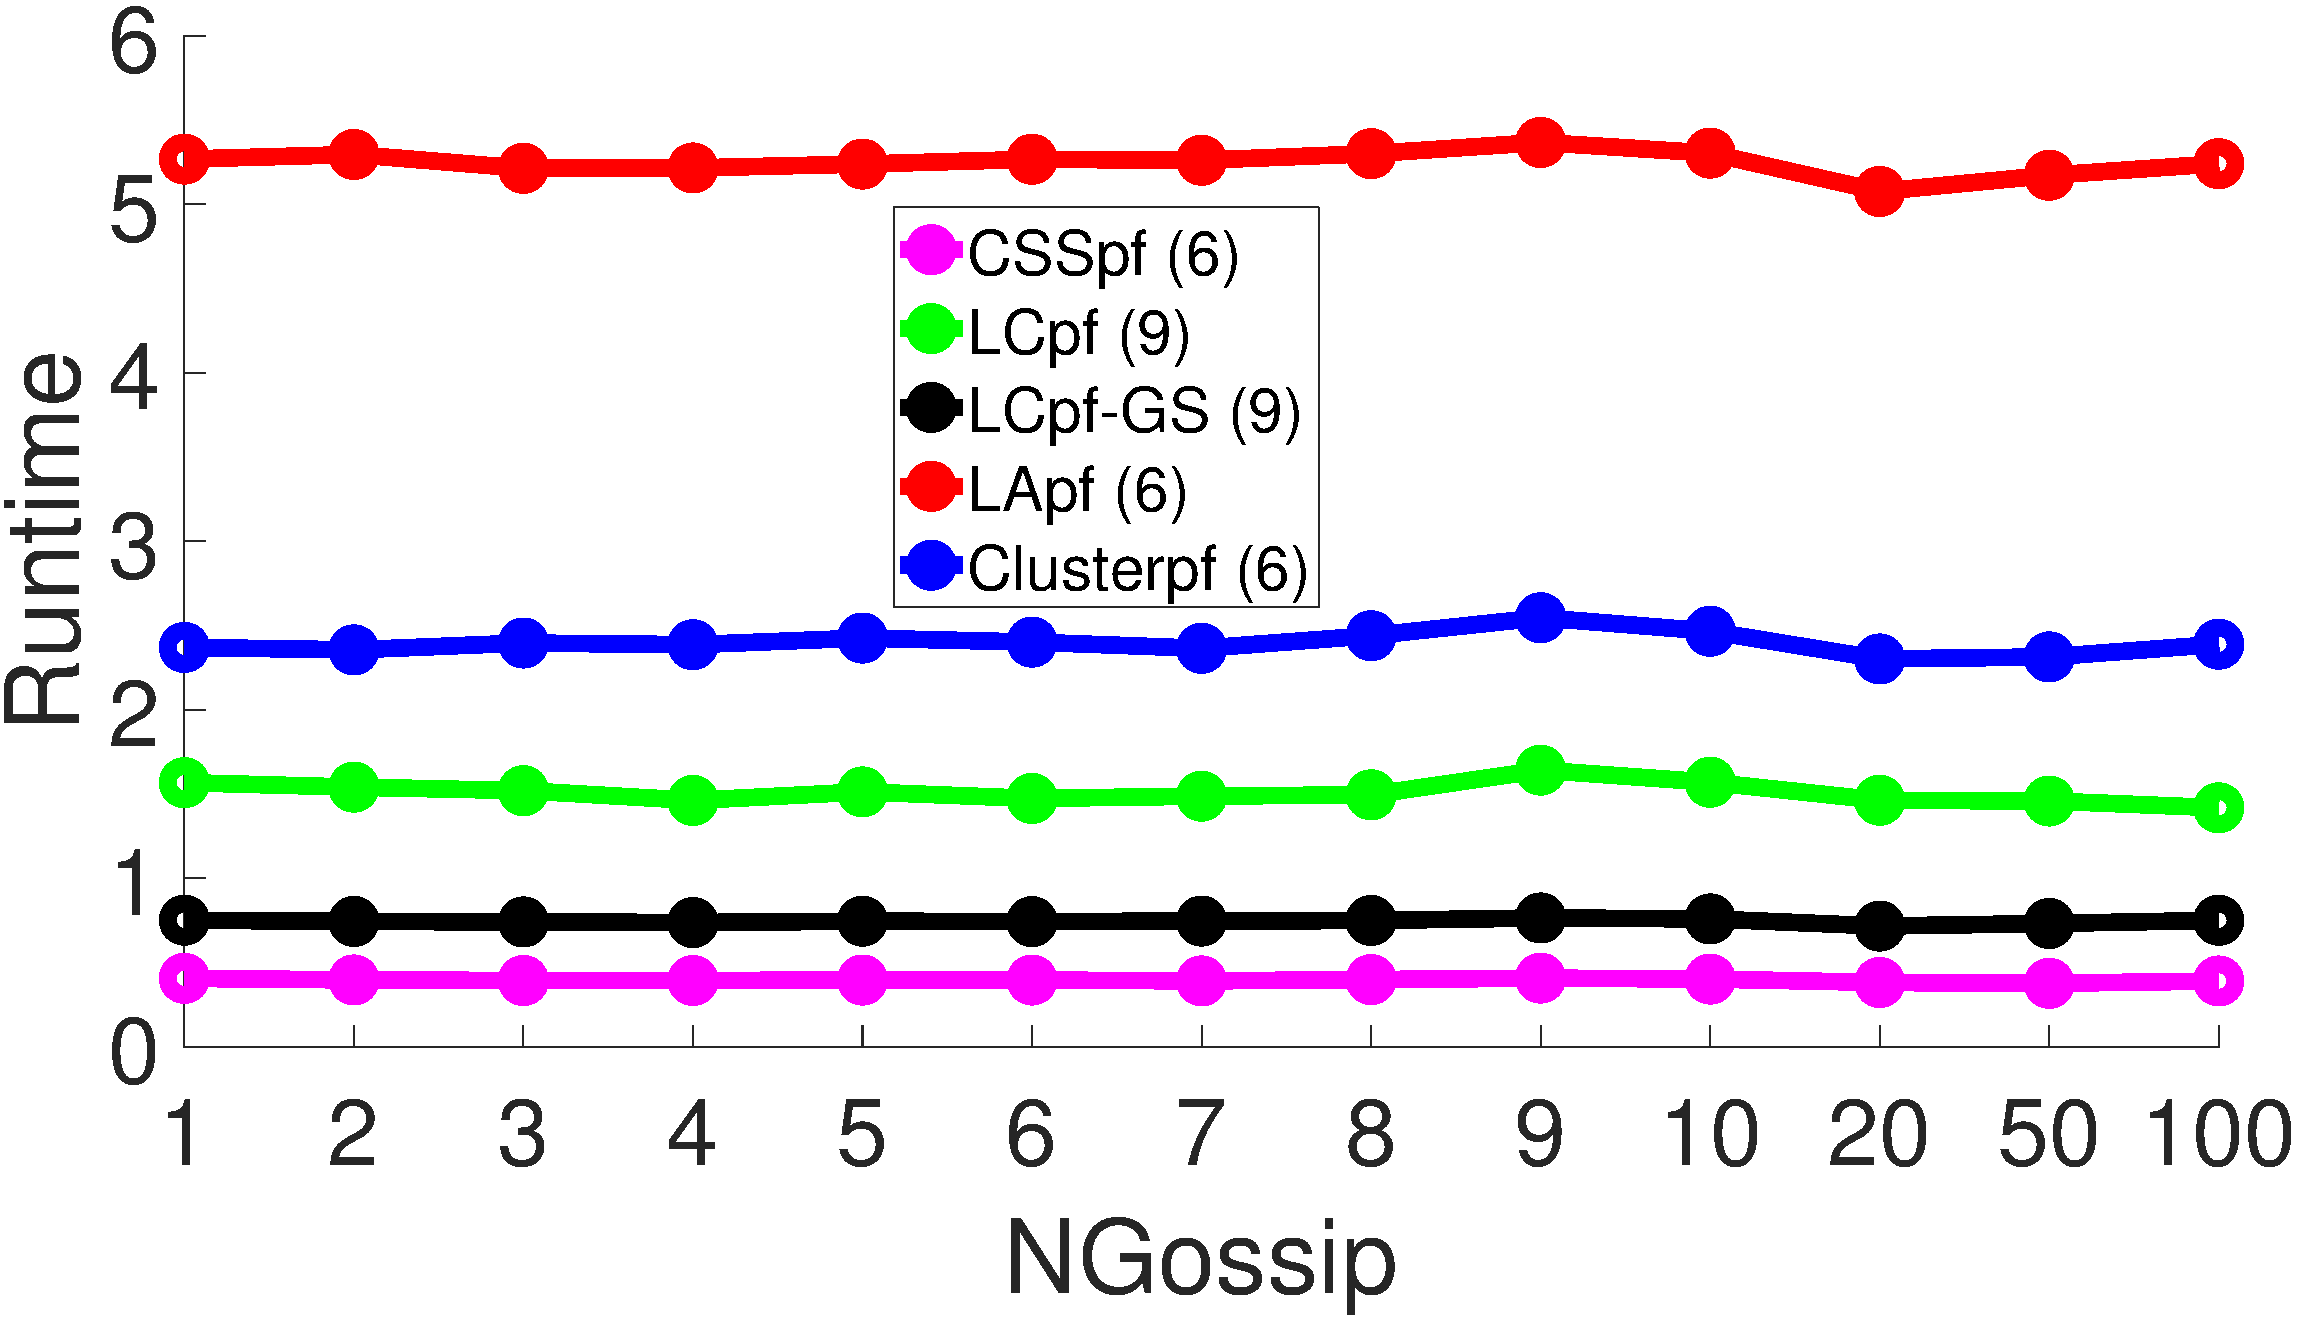
\includegraphics[width=0.45\textwidth]{Figures/Track1_time}}
\end{subfigure}
\begin{subfigure}[Track 2, Total runtime]
{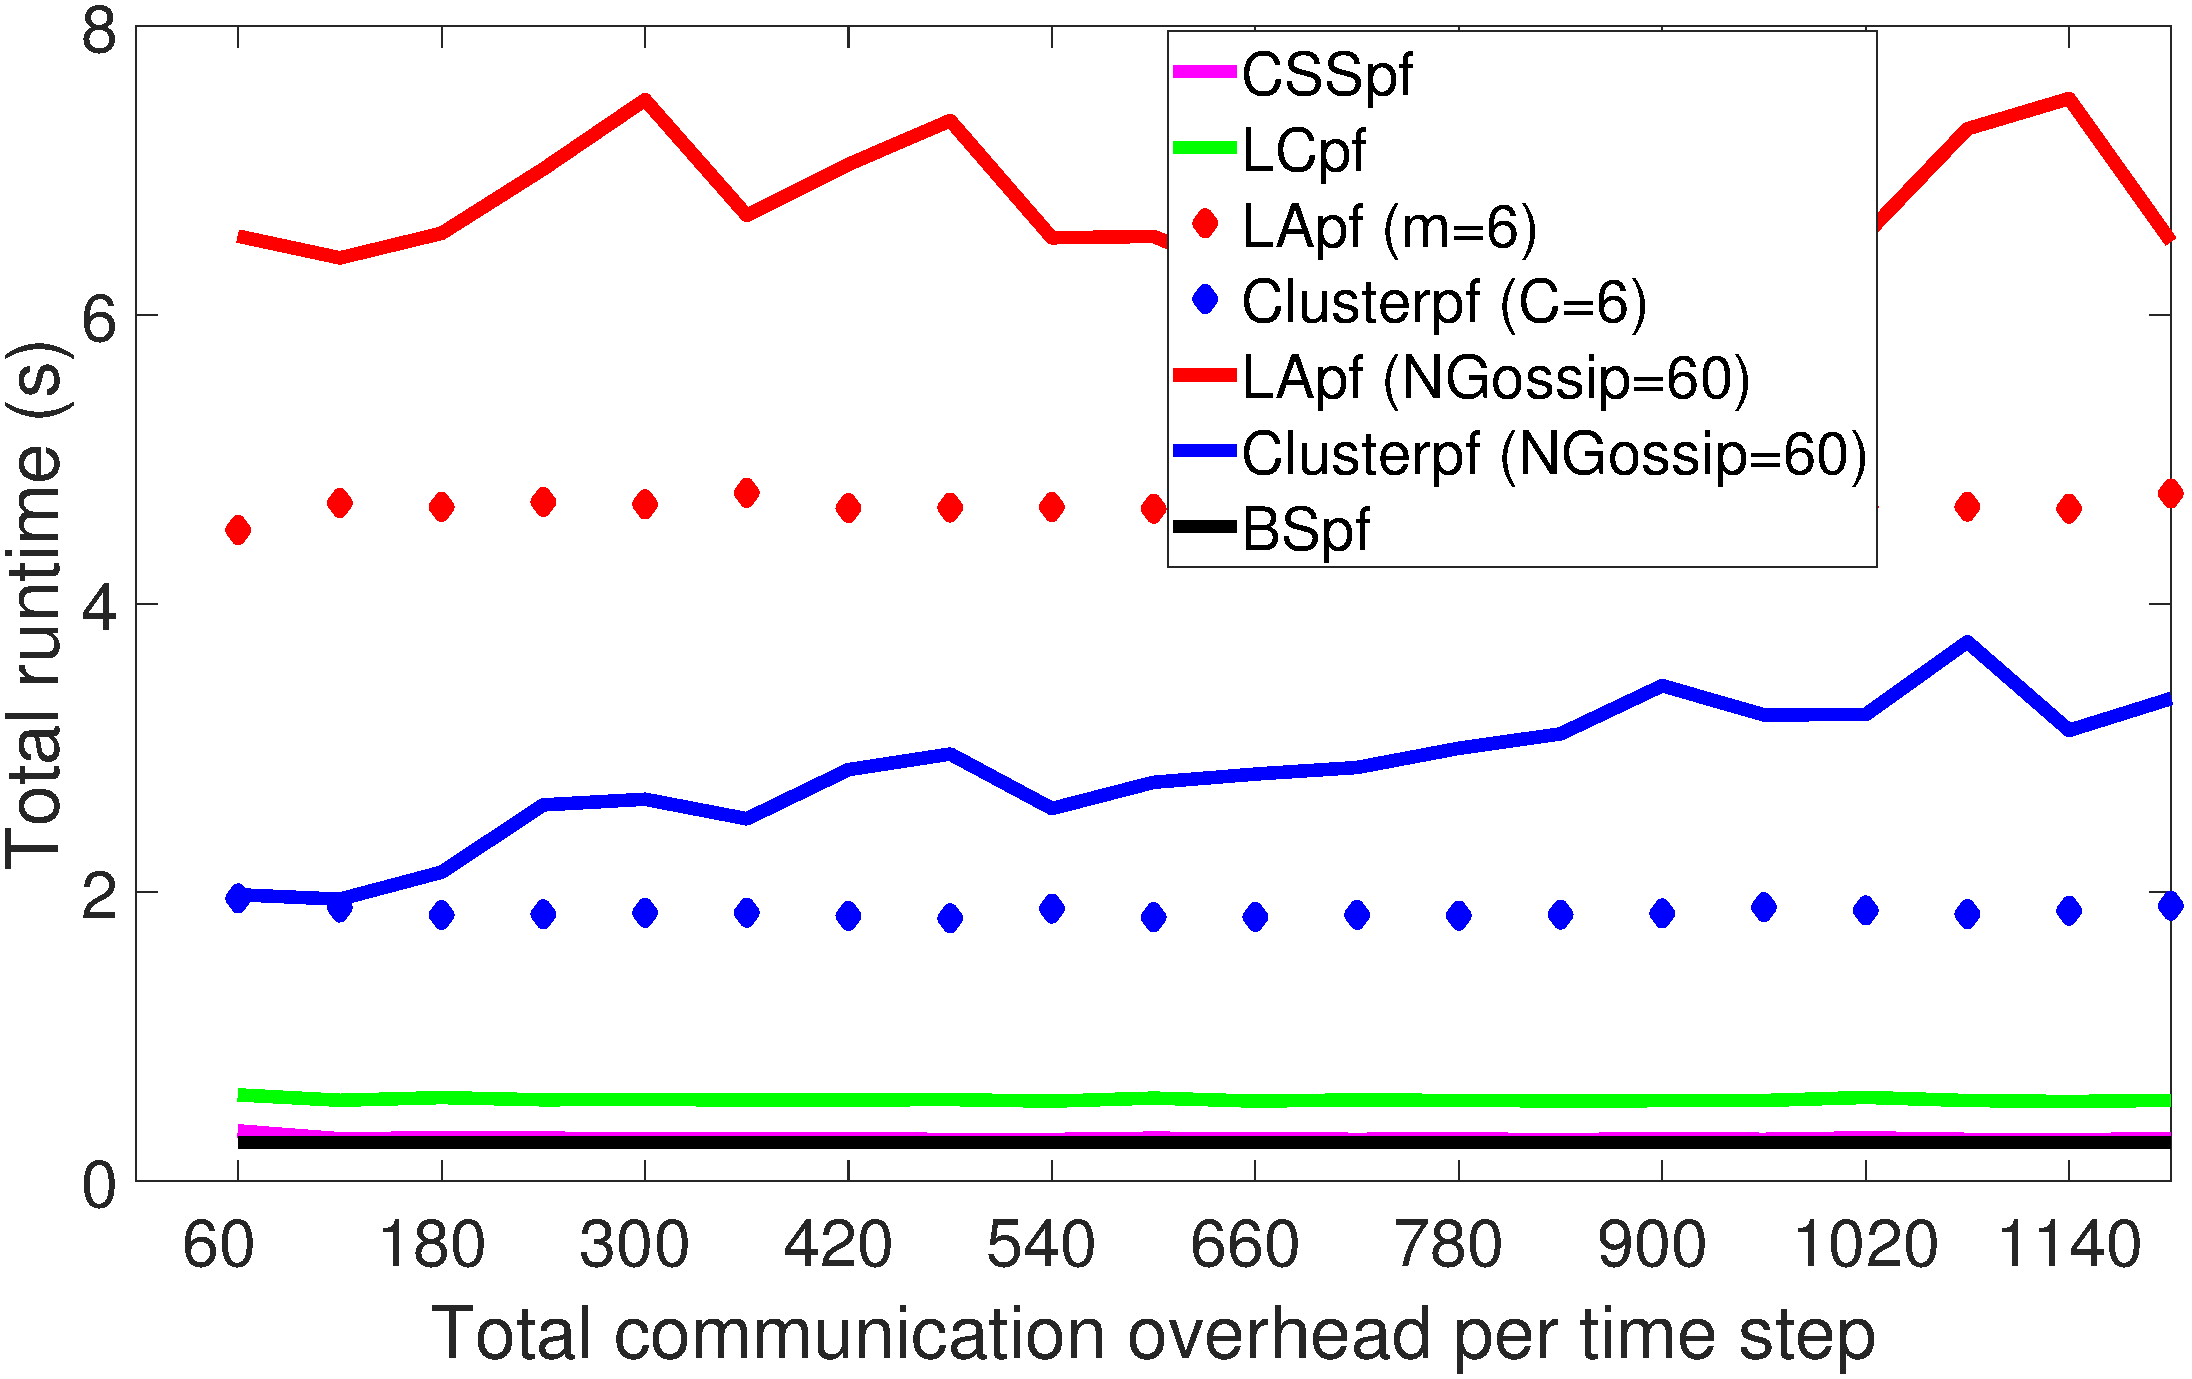
\includegraphics[width=0.45\textwidth]{Figures/Track2_time}}
\end{subfigure}
\caption{RMSE and total runtime, averaged over 200 Monte Carlo trials for test tracks 1 and 2. The number in brackets indicate the number of scalars broadcast per sensor per gossip iteration.}
\label{fig:simulation_results}
\end{figure}

%These simulation results suggest that our proposed filters, LApf and Clusterpf, are considerably less susceptible to gossiping noise than the other three distributed filters. We next conduct a sensitivity analysis of all filters. We run a centralized BSpf for both tracks. At each time step, we re-compute the posterior particle weights using all distributed filters. We then report the discrepancy of approximate and exact particle weights $||W_{BS}-W_{CSS}||_2$. The goal is to show each filter's susceptibility to gossiping error. Fig.~\ref{fig:weight_discrepancy} shows the results. For LApf and Clusterpf, the weight discrepancy never exceeds 0.1 (even at very low $NGossip$). For LCpf and CSSpf, the discrepancy remains high for low $NGossip$ and drops sharply after a threshold. These trends are consistent with the RMSE curves in the previous simulations. We do note that low weight discrepancy does not necessarily translate to low RMSE. LApf and Clusterpf have similar RMSE yet there is a clear gap in their weight discrepancy. The LCpf-GS has the lowest weight discrepancy for $NGossip\geq 6$; yet this does not translate to low RMSE. 

%\begin{figure}[h]
%\centering
%\begin{subfigure}[Track 1]
%{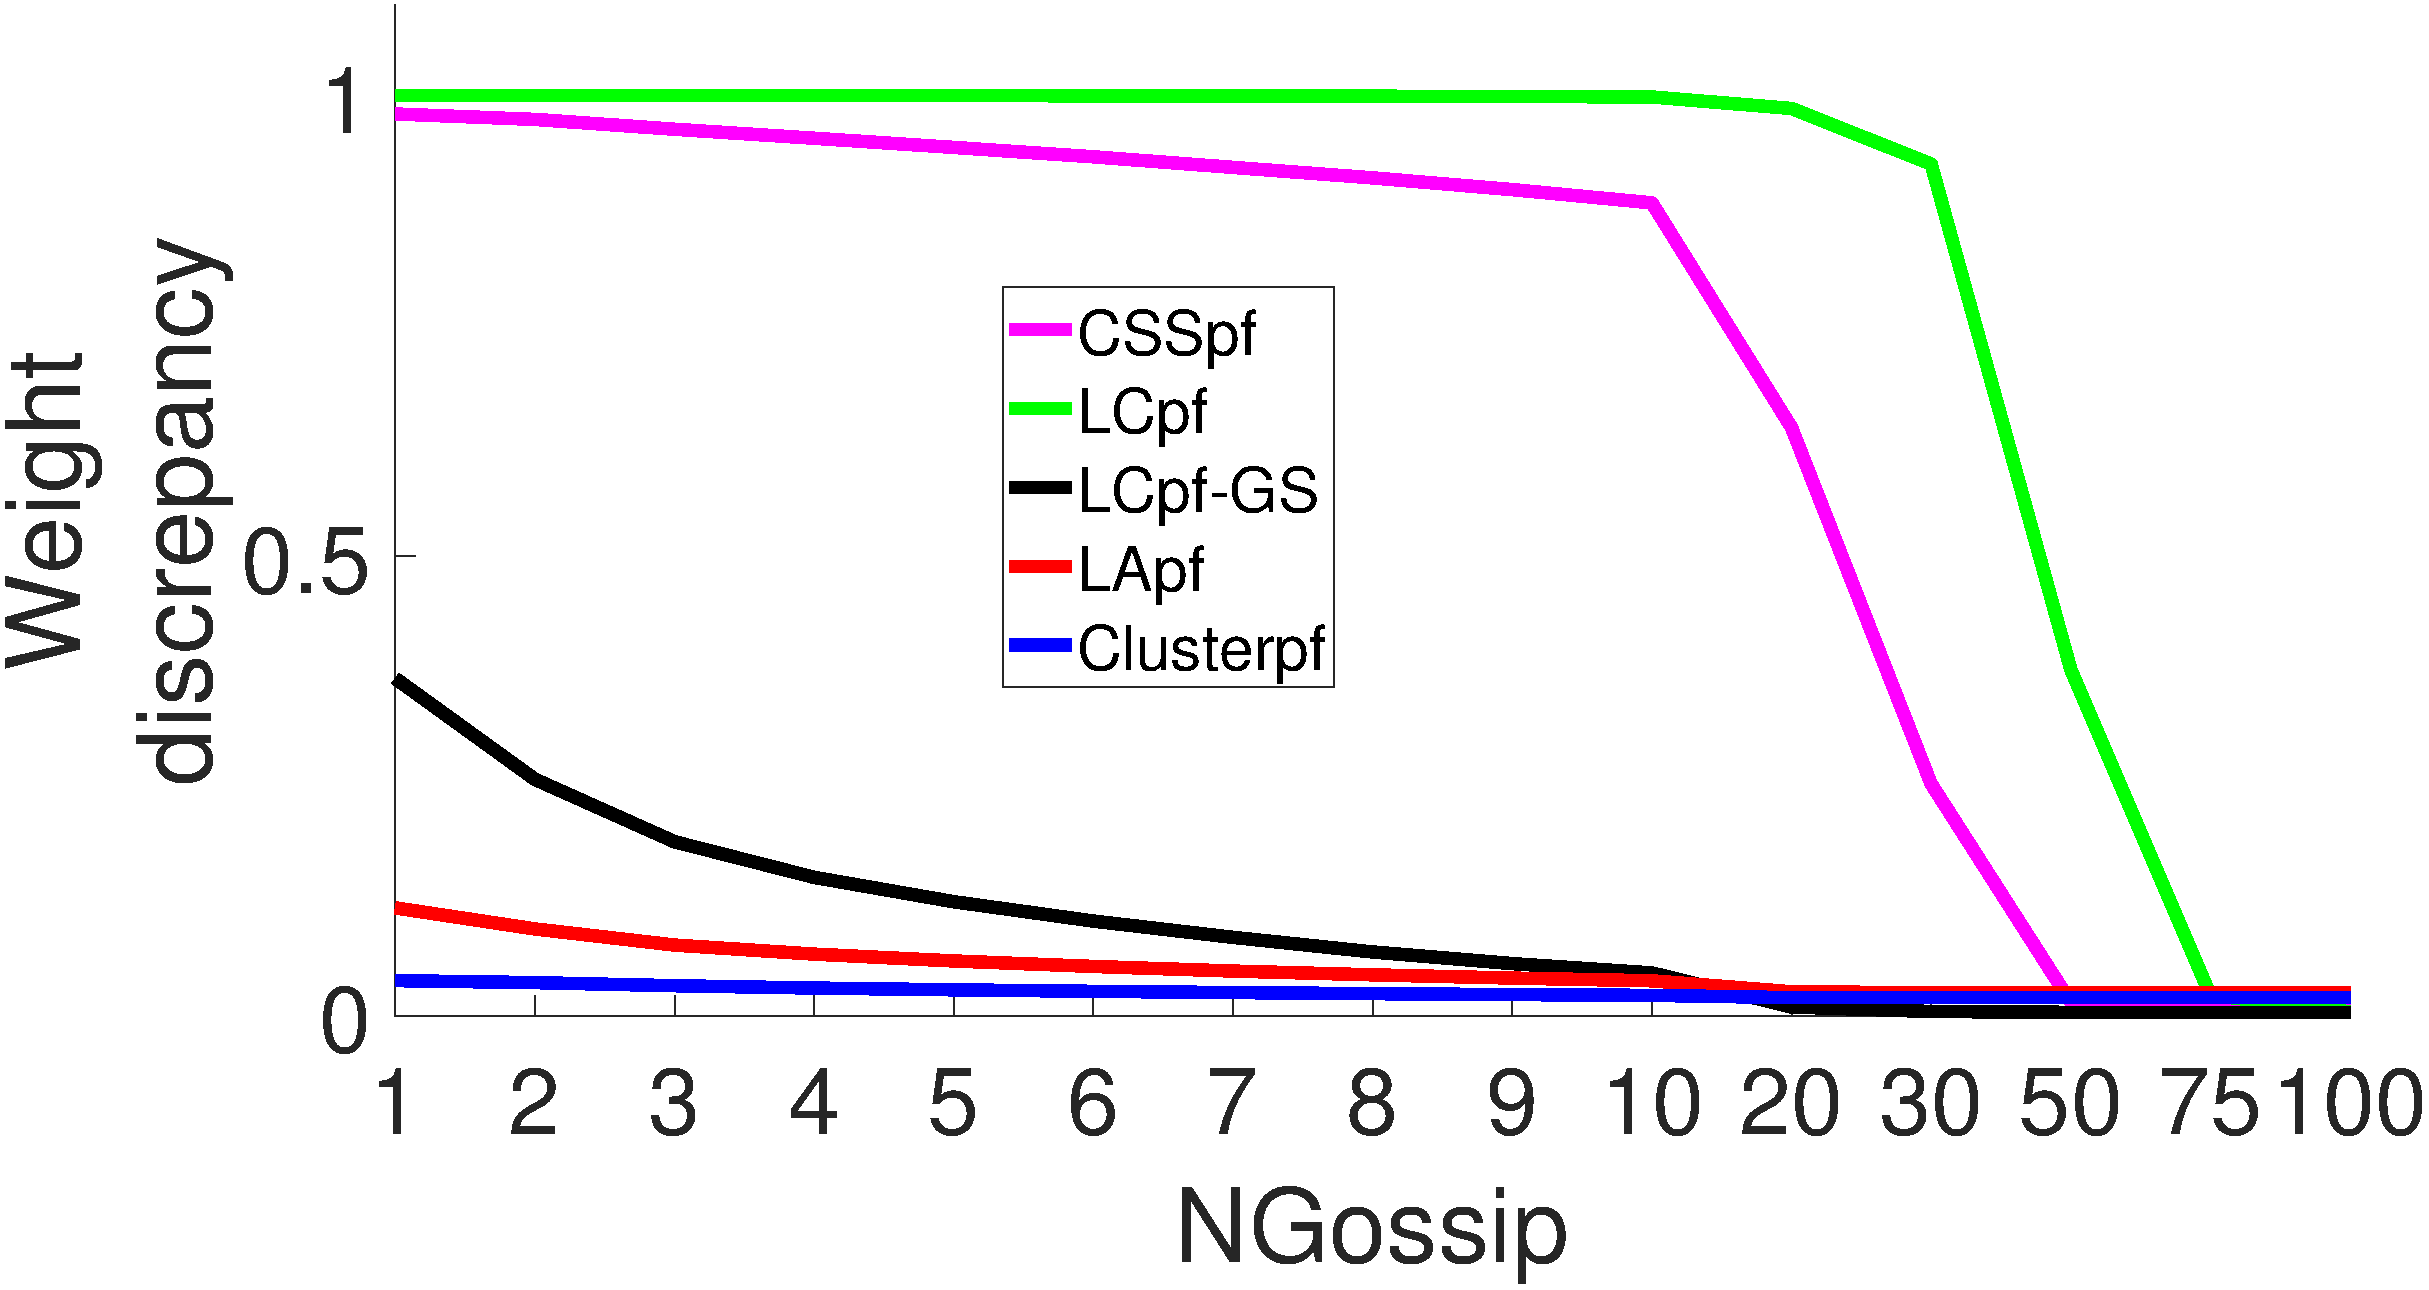
\includegraphics[width=0.45\textwidth]{Figures/Track1_weight_discrepancy}}
%\end{subfigure}
%\begin{subfigure}[Track 2]
%{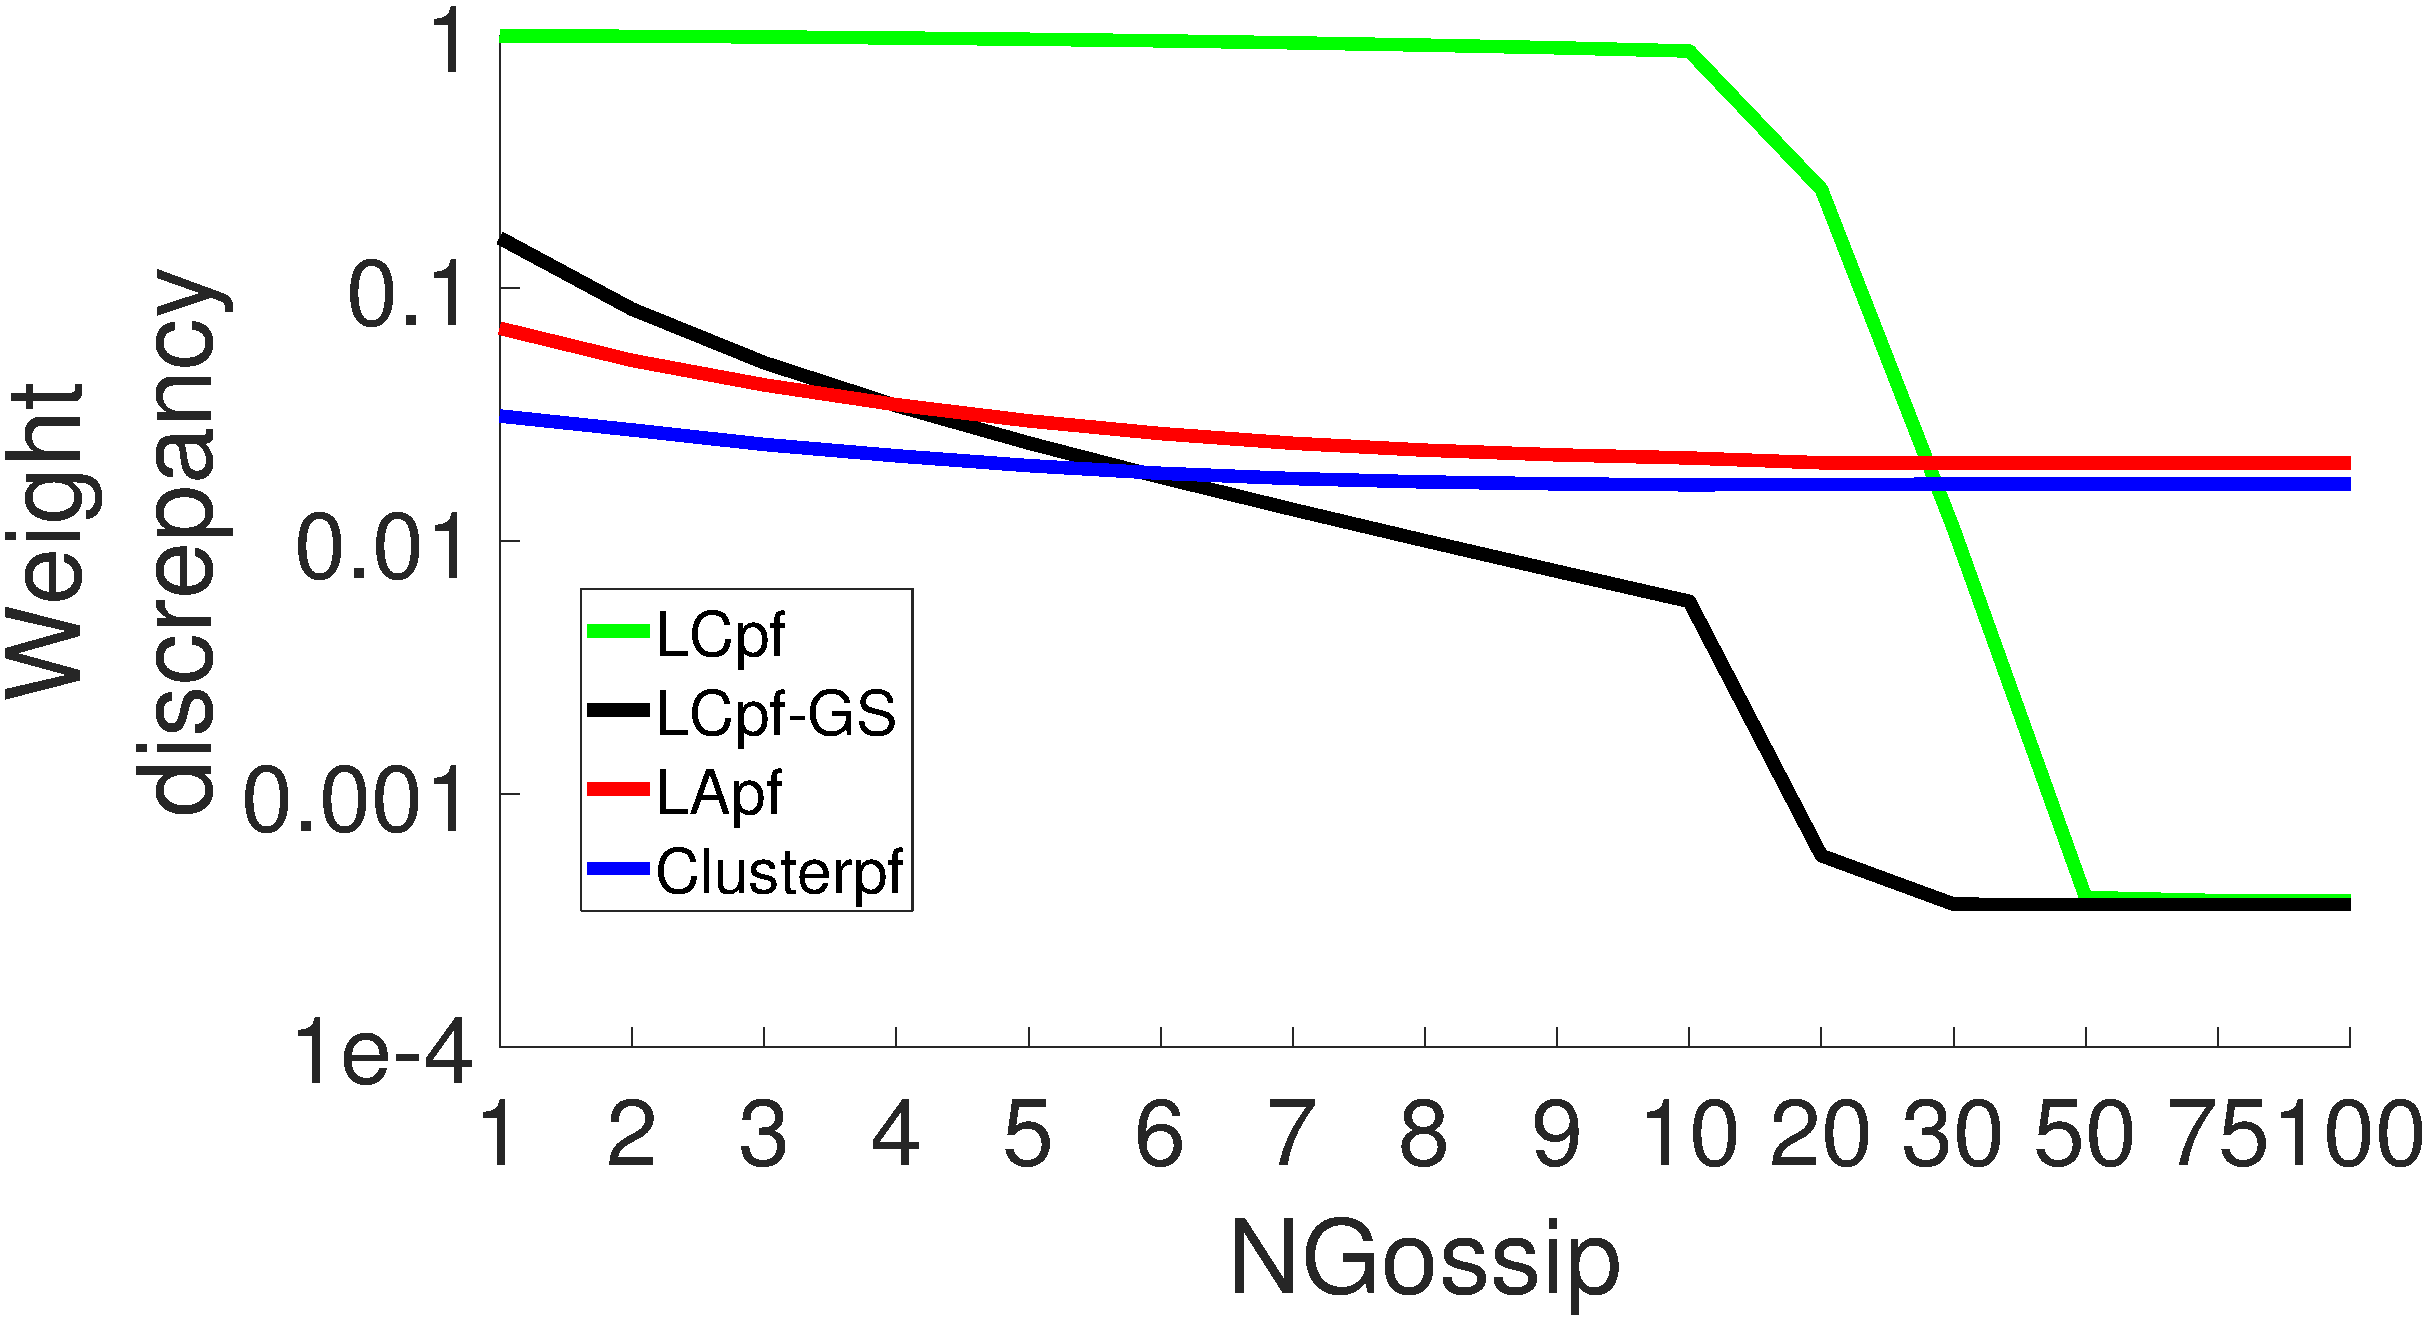
\includegraphics[width=0.45\textwidth]{Figures/Track2_weight_discrepancy}}
%\end{subfigure}
%\caption{Average weight discrepancy $||W_{BS}-W_{approx}||_2$ over time. The actual tracking is done using true particle weights.}
%\label{fig:weight_discrepancy}
%\end{figure}

\section{Theoretical analysis}
Let $\hat{\gamma}(X_i)$ denote the approximate joint particle log-likelihood for particle $X_i$ and let $\gamma(X_i)$ denote the exact value. In this section, our objective is to derive an upper bound for $\frac{||\hat{\gamma}(X_i)-\gamma(X_i)||}{||\gamma(X_i)||}$ and to understand the robustness of the proposed filters even at low gossiping iterations.

All distributed filters presented in the simulations follow the same general steps:
\begin{enumerate}
\item Each sensor computes local particle log-likelihoods.
\item Each sensor encodes the local log-likelihoods into $m$ coefficients.
\item Gossip and max-consensus algorithms are used to compute the $m$ aggregate coefficients. 
\item Approximate joint log-likelihoods are recovered from the aggregate coefficients. 
\end{enumerate}

Therefore, the discrepancy between true log-likelihoods $\gamma(x_i)$ and the final approximate value $\hat{\gamma}(x_i)$ comes from two sources: the encoding error and the gossiping error. The first error is the discrepancy between true log-likelihoods and its reconstructions using $m$ coefficients. The second error occurs when sensors do not obtain the true aggregate coefficient values after only a finite number of gossiping iterations. 

Consider the encoding error first. Let $\gamma_m(X_i)$ denote the approximate log-likelihood recovered from $m$ coefficients. We assume that the following bound on encoding error holds for all particles $X_i$
\begin{equation}
|\gamma_{m}(X_i) - \gamma(X_i)|\leq \delta_m|\gamma(X_i)| 
\label{eqn:encoding_error}
\end{equation}

%We can derive the following bound on the entire log-likelihood vector
%\begin{align}
%\frac{||\gamma_{m} - \gamma||}{||\gamma||} &= \frac{||\Psi(\Psi^T\Psi)^{-1}\Psi^T\gamma - \gamma||}{||\gamma||} \nonumber \\
%&\leq ||\Psi(\Psi^T\Psi)^{-1}\Psi^T-I||
%\label{eqn:encoding_error_vector}
%\end{align}
%where $I$ is the identify matrix of appropriate dimension

%We assume that the following bound on encoding error holds for all particles $x_i$
%\begin{equation}
%|\gamma_{m}(x_i) - \gamma(x_i)|\leq \delta_m|\gamma(x_i)| 
%\label{eqn:encoding_error}
%\end{equation}

%With suitable normalization, we have $\gamma(x_i)\leq 0 \quad \forall x_i$ so that the right hand of Eq.~\eqref{eqn:encoding_error} is always positive. 

The ratio term $0\leq \delta_m\leq 1$ depends on the specific filter and the number of coefficients $m$. Given a required threshold $\delta_m$, each sensor can choose a suitable value of $m$; then max-consensus algorithm can be used to agree on a network-wide value. Note that Eq.~\eqref{eqn:encoding_error} can be rewritten to yield
\begin{equation}
(1-\delta_m)|\gamma(X_i)| \leq |\gamma_m(X_i)| \leq (1+\delta_m)|\gamma(X_i)|
\end{equation}

Consider the gossiping error. Let $\hat{\alpha}$ denote the coefficients obtained after gossiping and max-consensus iterations. This gives us the approximate log-likelihoods $\hat{\gamma}$. We seek to establish the following error ratio
\begin{equation}
\frac{|\gamma_m(X_i)-\hat{\gamma}(X_i)|}{|\gamma_m(X_i)|} \leq \delta_{Gossip}
\label{eqn:gossiping_error}
\end{equation}

Putting everything together, we obtain
\begin{align}
\frac{|\hat{\gamma}(X_i) - \gamma(X_i)|}{|\gamma(X_i)|}&=\frac{|\hat{\gamma}(X_i) -\gamma_m(X_i) + \gamma_m(X_i) - \gamma(X_i)|}{|\gamma(X_i)|} \\
&\leq \frac{|\hat{\gamma}(X_i) -\gamma_m(X_i)|}{|\gamma(X_i)|}+\frac{|\gamma_m(X_i) - \gamma(X_i)|}{|\gamma(X_i)|} \\
&\leq (1+\delta_m)\frac{|\hat{\gamma}(X_i) -\gamma_m(X_i)|}{|\gamma_m(X_i)|}+\frac{|\gamma_m(X_i) - \gamma(X_i)|}{|\gamma(X_i)|} \\
&\leq (1+\delta_m)\delta_{gossip} + \delta_m  = \delta
\label{eqn:error_bound}
\end{align}

Consider Eq.~\eqref{eqn:error_bound}. When both the encoding and gossiping errors are present, they have a cascading effect on the overall error propagation. The overall error is bounded (i.e., less than unity) when both terms are bounded and less than unity. In fact, $\delta\leq 1$ is one of the conditions required to establish a time-uniform bound on the overall error of particle filters~\cite{Syamantak2015}. The other conditions are
\begin{enumerate}
\item The Markov chain associated with target state transition undergoes sufficient mixing within a finite number of time steps. 
\item The state estimate function $F(X_i)$ can be suitably scaled and bounded such that $\sup_{X_i} |F(X_i)|<1$
\item The likelihoods is bounded $\exp(\gamma(X_i))\leq 1 \quad \forall X_i$. 
\end{enumerate}
Note the fulfilling the first two conditions is independent of the choice of the filter. The third condition can be easily satisfied with suitable normalization of log-likelihoods. Thus  our discussion focuses only on the error bound $\delta$. More specifically, we focus on $\delta_{\text{gossip}}$ since $\delta_m$ can be reduced by simply increasing the number of coefficients. 

Let $\hat{\alpha}(l)$ be the coefficients obtained after $l$ gossip iterations and max-consensus iterations and let $\alpha$ denote the true coefficient values. We seek to establish the following bound for all coefficients:
\begin{equation}
\frac{|\hat{\alpha}_j(l)-\alpha_j|}{|\alpha_j|}\leq \beta, \quad 1\leq j\leq m
\label{eqn:gossip_bound}
\end{equation}
Let $S$ denote the total number of sensors, let $W$ denote the $S\times S$ averaging matrix used in the gossiping algorithm and let $\rho_W$ denote its second largest eigenvalue in modulus. The bound in Eq.~\eqref{eqn:gossip_bound} holds if the minimum number of gossip iteration satisfies the following condition~\cite{Olshevsky2009}
\begin{equation}
l\geq \frac{1.5\log(S)+\log(\frac{S-1}{\beta})}{\log(1/\rho_W)}
\label{eqn:minimum_NGossip}
\end{equation}

For CSSpf, LCpf, LCpf-GS and LApf, we can define a linear transformation between between the coefficients $\alpha$ and the approximate log-likelihoods $\hat{\gamma}$. For CSSpf and LCpf which use $m$ basis functions for encoding, we have the $N\times m$ matrix $\Psi_{LC/CSS}$ where $\Psi(i,j)=\beta_j(X_i)$. For LCpf-GS, we start with the same matrix $\Psi_{LC}$ and apply Gram-Schmidt process to obtain an orthonormal matrix $\Psi_{LC-GS}$. For LApf, the matrix $\Psi_{LA}$ simply contains the $m$ eigenvectors corresponding to the $m$ smallest eigenvalues of the graph Laplacian. Finally, for Clusterpf, the cluster assignment matrix $C$ can be interpreted as an encoding matrix; although the reverse process is not a linear transformation which complicates the analysis. To summarize, we have
\begin{align}
\gamma_m^{\text{CSS}} &= \Psi^{\text{CSS}}\alpha^{\text{CSS}}\\
\gamma_m^{\text{LC}} &= \Psi^{\text{LC}}\alpha^{\text{LC}} \\
\gamma_m^{\text{LC-GS}} &= \Psi^{\text{LC-GS}}\alpha^{\text{LC-GS}} \\
\gamma_m^{\text{LA}} &= \Psi^{\text{LA}}\alpha^{\text{LA}} \\
\gamma_m^{\text{LC}} &= \Psi^{\text{LC}}\alpha^{\text{LC}} \\
\gamma_m^{\text{Cluster}} &= \arg \min_{\gamma} \gamma^T L \gamma \quad C\gamma = \alpha^{\text{LC}} 
\end{align}

%Consider LApf, LCpf, LCpf-GS and CSSpf. Let $\Psi_i$ denote the $i^{th}$ row of encoding matrix $\Psi$ and let $\Psi_{ij}$ denote the $j^{th}$ entry of row vector $\Psi_i$. We can derive an upper bound for the gossiping error as follows: 

%\begin{align}
%|\hat{\gamma}(x_i)-\gamma_m(x_i)| &= \left\vert\sum_{j=1}^m \Psi_{ij}(\hat{\alpha}_j-\alpha_j)\right\vert \nonumber \\
%&\leq \sum_{j=1}^m\left\vert \Psi_{ij}(\hat{\alpha}_j-\alpha_j)\right\vert\nonumber  \\
%&\leq \sum_{j=1}^m\left\vert \Psi_{ij}\right\vert \phantom{1} \left\vert\hat{\alpha}_j-\alpha_j\right\vert \nonumber \\
%&\leq \beta\sum_{j=1}^m\left\vert \Psi_{ij}\right\vert \phantom{1} \left\vert\alpha_j\right\vert
%\end{align}
%where the first inequality follows from triangle inequality and the last inequality follows from Eq.31. 

%Dividing both sides by $|\gamma_m(x_i)|$ yields:
%\begin{align}
%\frac{|\hat{\gamma}(x_i)-\gamma_m(x_i)|}{|\gamma_m(x_i)|} &\leq  \frac{\beta \sum_{j=1}^m\left\vert \Psi_{ij}\right\vert \phantom{1} \left\vert\alpha_j\right\vert}{|\gamma_m(x_i)|} \nonumber\\
%&\leq \frac{\sum_{j=1}^m\beta \left\vert \Psi_{ij}\right\vert \left\vert\alpha_j\right\vert}{|\gamma(x_i)(1-\delta_m)|} \nonumber \\
%&\leq \frac{\sum_{j=1}^m\beta \left\vert \Psi_{ij}\right\vert \left\vert\alpha_j\right\vert}{\min_{x_i}|\gamma(x_i)(1-\delta_m)|} 
%%\delta_{\text{gossip}}
%\label{eqn:gossiping_error}
%\end{align}

%Consider first the numerator in Eq.~\eqref{eqn:gossiping_error}. Higher value of $\beta$ suggests higher error in aggregated coefficients and increases $\delta_{\text{gossip}}$ as expected. More interestingly, both $|\Psi_{ij}|$ and $|\alpha_j|$ also increase $\delta_{\text{gossip}}$. This matches our observations that filters using orthonormal encoding matrix require lower communication overhead. In the denominator, lower encoding error $\delta_m$ reduces $\delta_{\text{gossip}}$. 

%An alternate bound can be derived from the infinity norm:
We can derive an upper bound for the gossiping error of CSSpf, LCpf, LCpf-GS and LApf as follows: 
\begin{align}
\frac{|\hat{\gamma}(X_i)-\gamma_m(X_i)|}{|\gamma_m(X_i)|} &\leq  \frac{||\hat{\gamma}-\gamma ||_\infty}{|\gamma_m(X_i)|} \nonumber \\
&= \frac{||\Psi (\hat{\alpha}-\alpha) ||_\infty}{|\gamma_m(x_i)|} \nonumber \\
&\leq \frac{||\Psi||_\infty ||\hat{\alpha}-\alpha ||_\infty}{(1-\delta_m)|\gamma(x_i)|} \nonumber \\
&\leq \frac{\beta ||\Psi||_\infty ||\alpha ||_\infty}{(1-\delta_m)\min_{x_i}|\gamma(x_i)|} 
\label{eqn:gossiping_error2}
\end{align}
where the third line follows from triangular inequality and Eq.~\eqref{eqn:encoding_error} and the last line follows from Eq.~\eqref{eqn:gossip_bound}. 

To validate the derived error bounds, we run the following simulations. We run a centralized bootstrap filter. At each time step, for comparison, we re-compute the particle weights using all the distributed filters. We compute and report the following the values:
\begin{enumerate}
\item $\max_{X_i} \frac{|\gamma_{m}(X_i)-\gamma(X_i)|}{|\gamma(X_i)|}$: estimate of $\delta_m$
\item $\max_{x_i} \frac{|\gamma_m(X_i)-\hat{\gamma}(X_i)|}{|\gamma_m(X_i)|}$: estimate of $\delta_{gossip}$ 
\item $\max_{\alpha_j} \frac{\left\vert \hat{\alpha}_j -\alpha_j \right\vert}{|\alpha_j|}$: estimate of $\beta$
\item $\frac{\beta ||\Psi||_\infty ||\alpha||_\infty}{\min_{x_j}|\gamma(x_j)(1-\delta_m)|}$: upper limit of $\delta_{gossip}$ for LApf, LCpf, LCpf-GS and CSSpf
\item $\max_{x_i} \frac{|\hat{\gamma}(x_i) - \gamma(x_i)|}{|\gamma(x_i)|}$: estimate of $\delta$
\item $(1+\delta_m)\delta_{gossip} + \delta_m$: upper limit of $\delta$
\item $||w_{true}-w_{approx}||_2$: discrepancy of normalized particle weights
\end{enumerate} 

\begin{figure}
\centering
\begin{subfigure}[Encoding error $\delta_m$]
{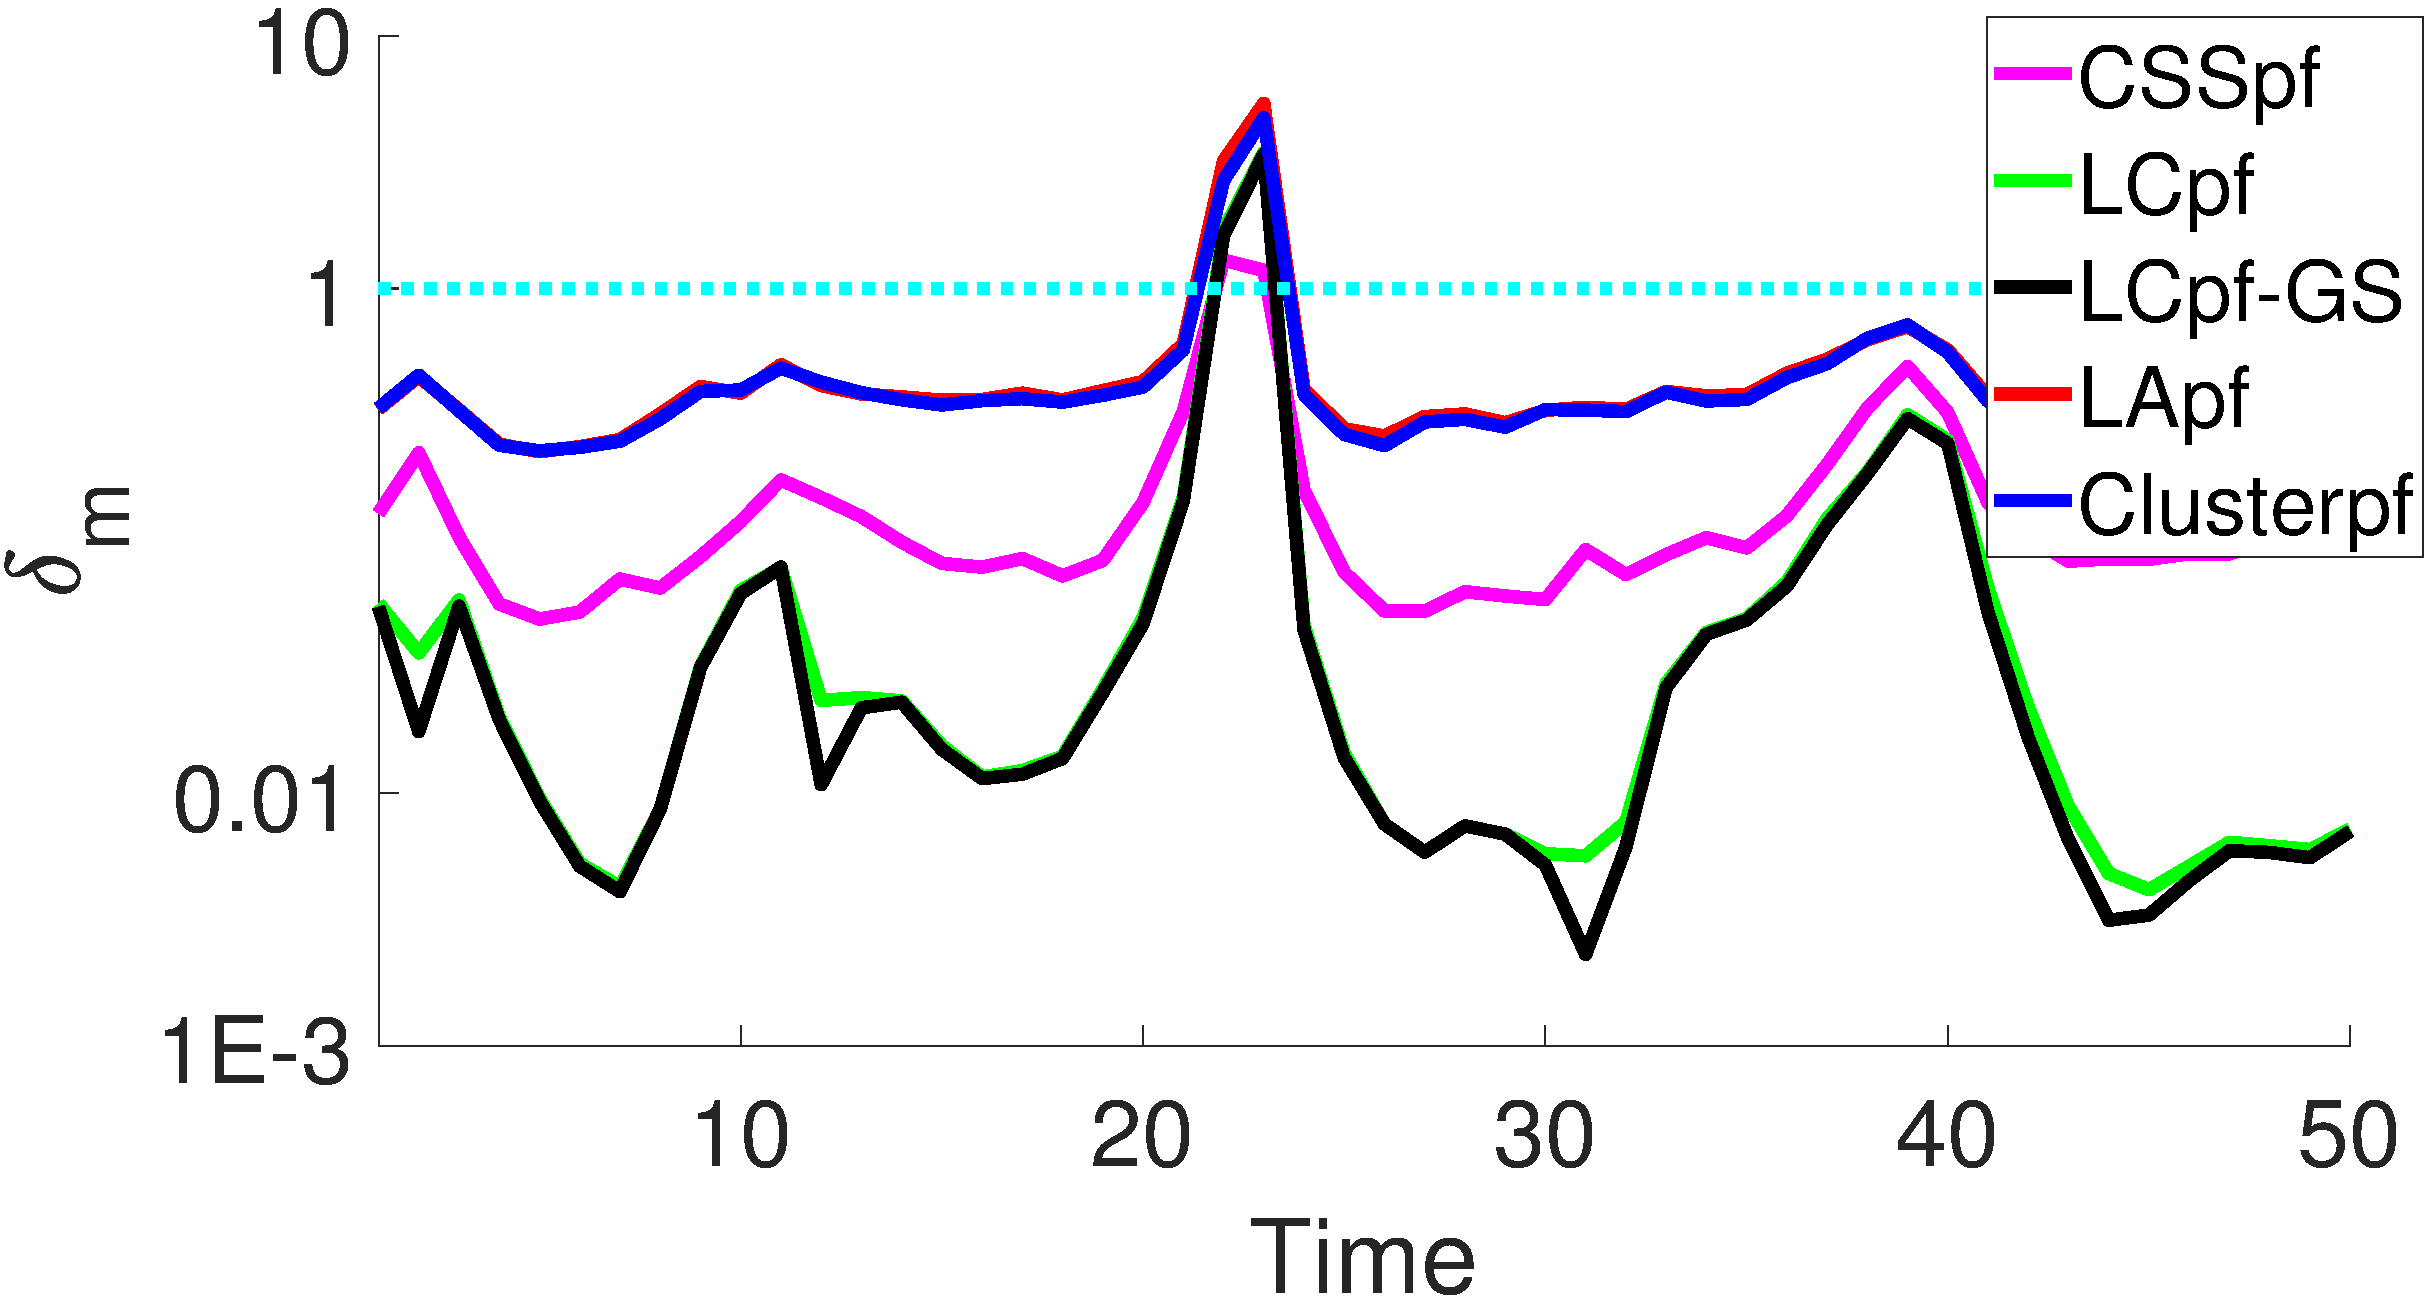
\includegraphics[width=0.49\textwidth]{Figures/delta_m_time_track2}}
\end{subfigure}
\begin{subfigure}[Gossiping error $\delta_{\text{gossip}}$, circles represent true gossiping errors and sold lines represent the theoretical upper bound based on infinity norm]
{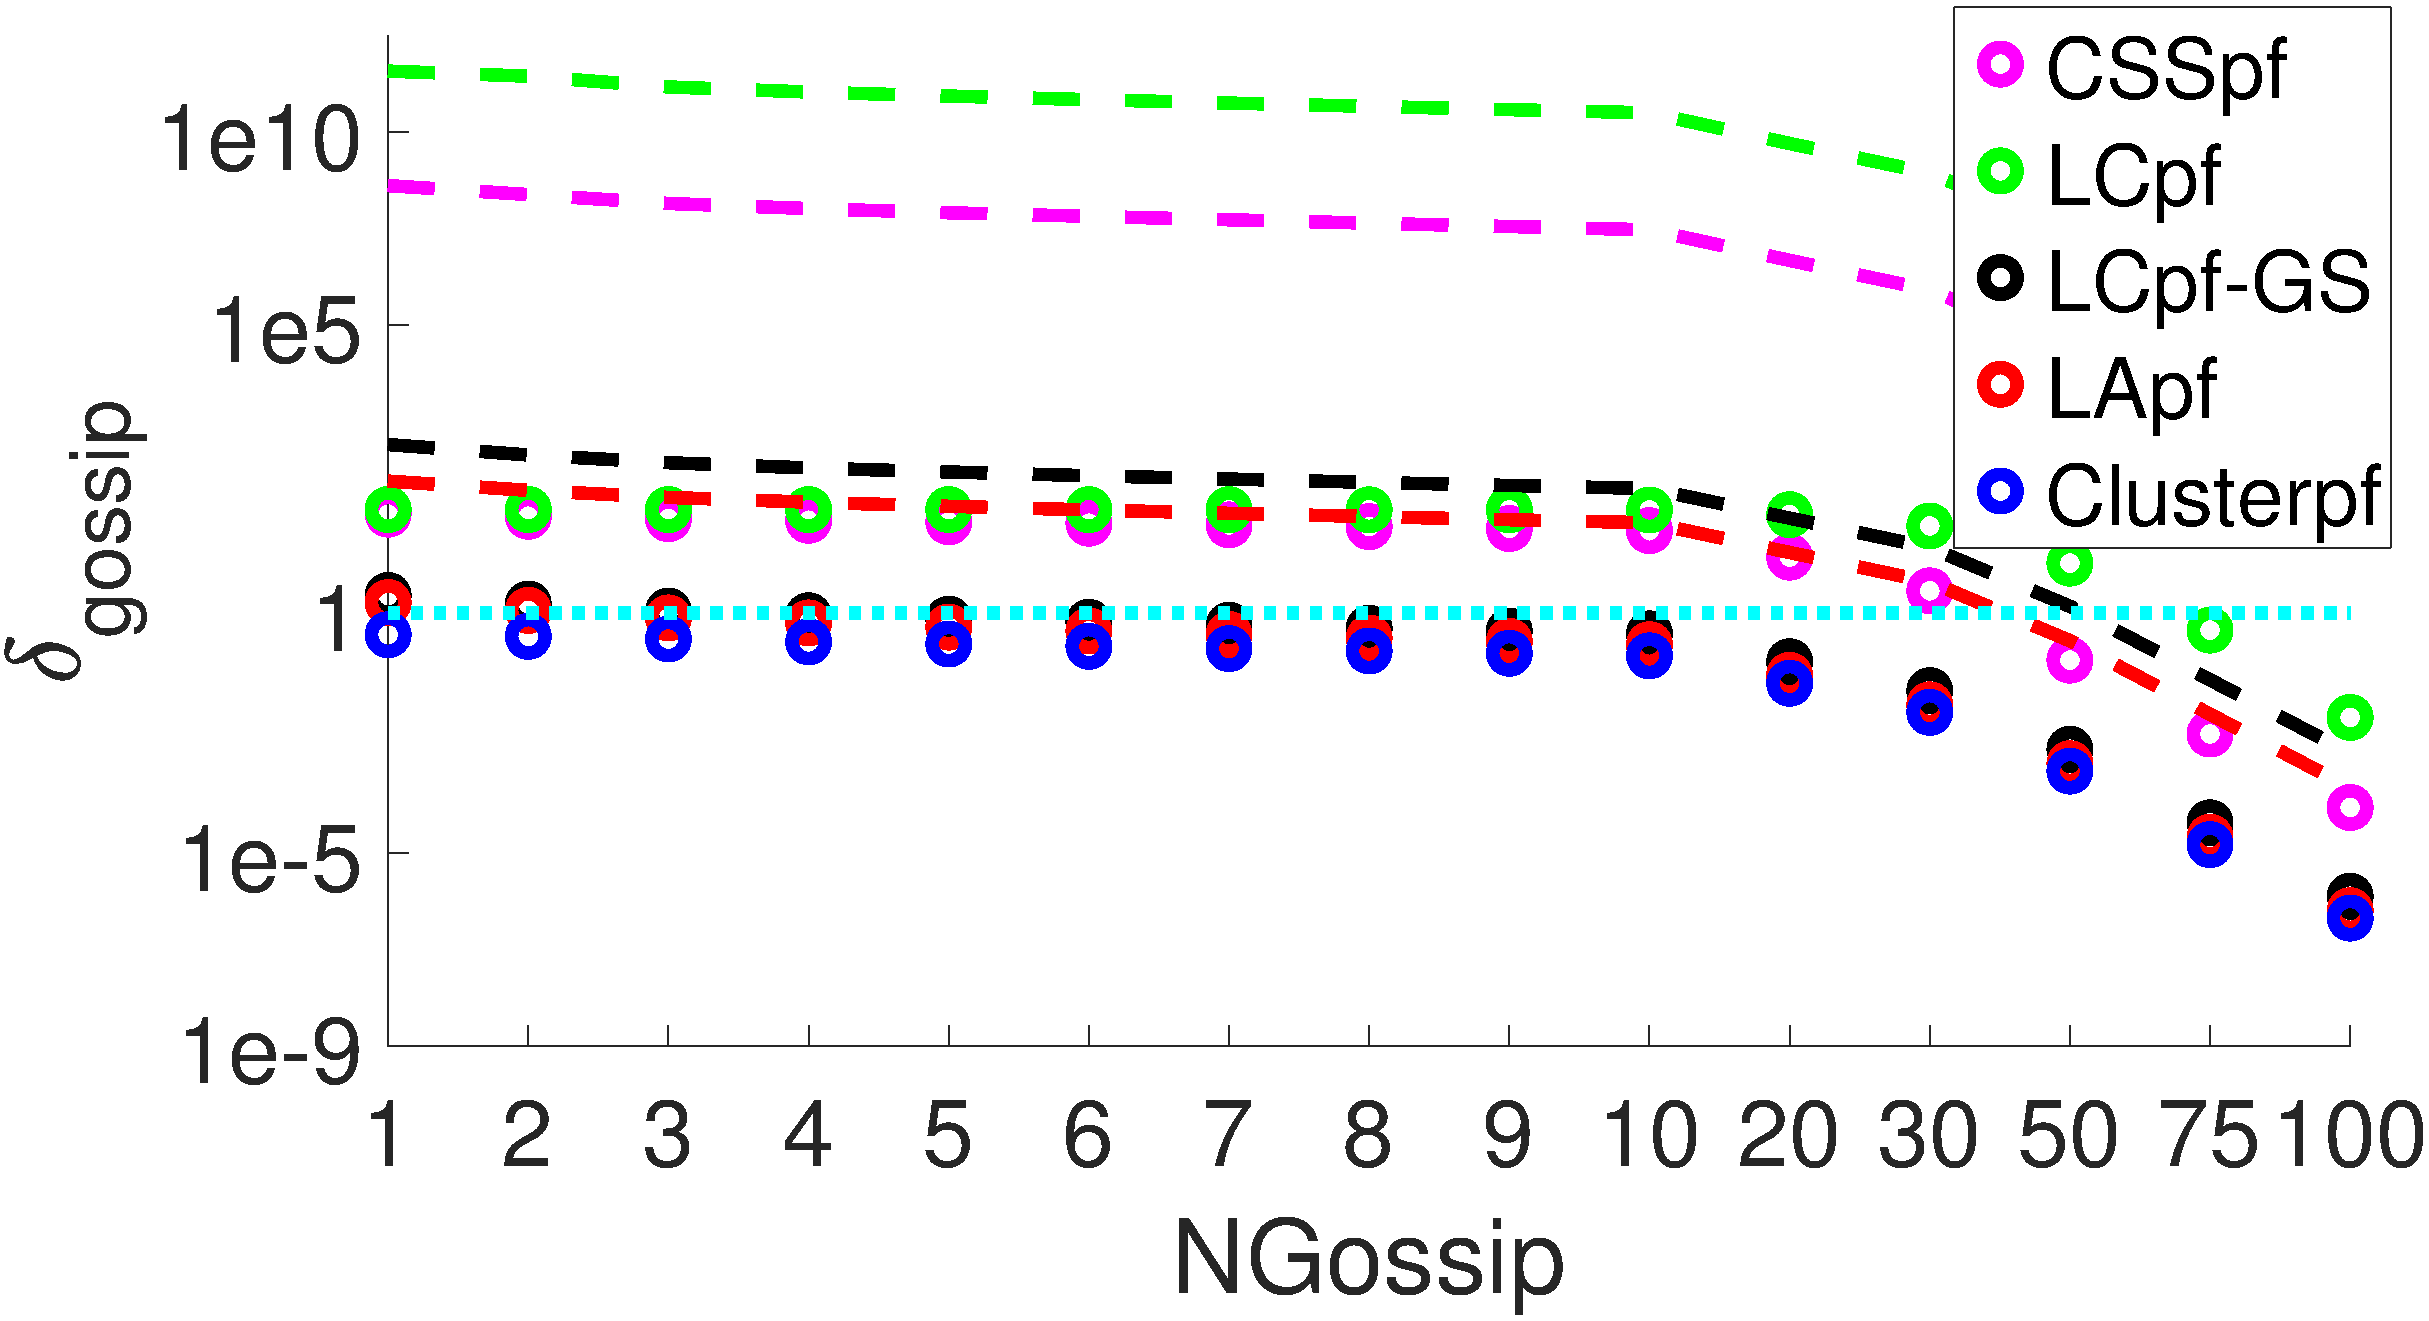
\includegraphics[width=0.49\textwidth]{Figures/delta_gossip2_track2}}
\end{subfigure}
\begin{subfigure}[$\beta$, the error ratio of coefficients $\alpha$]
{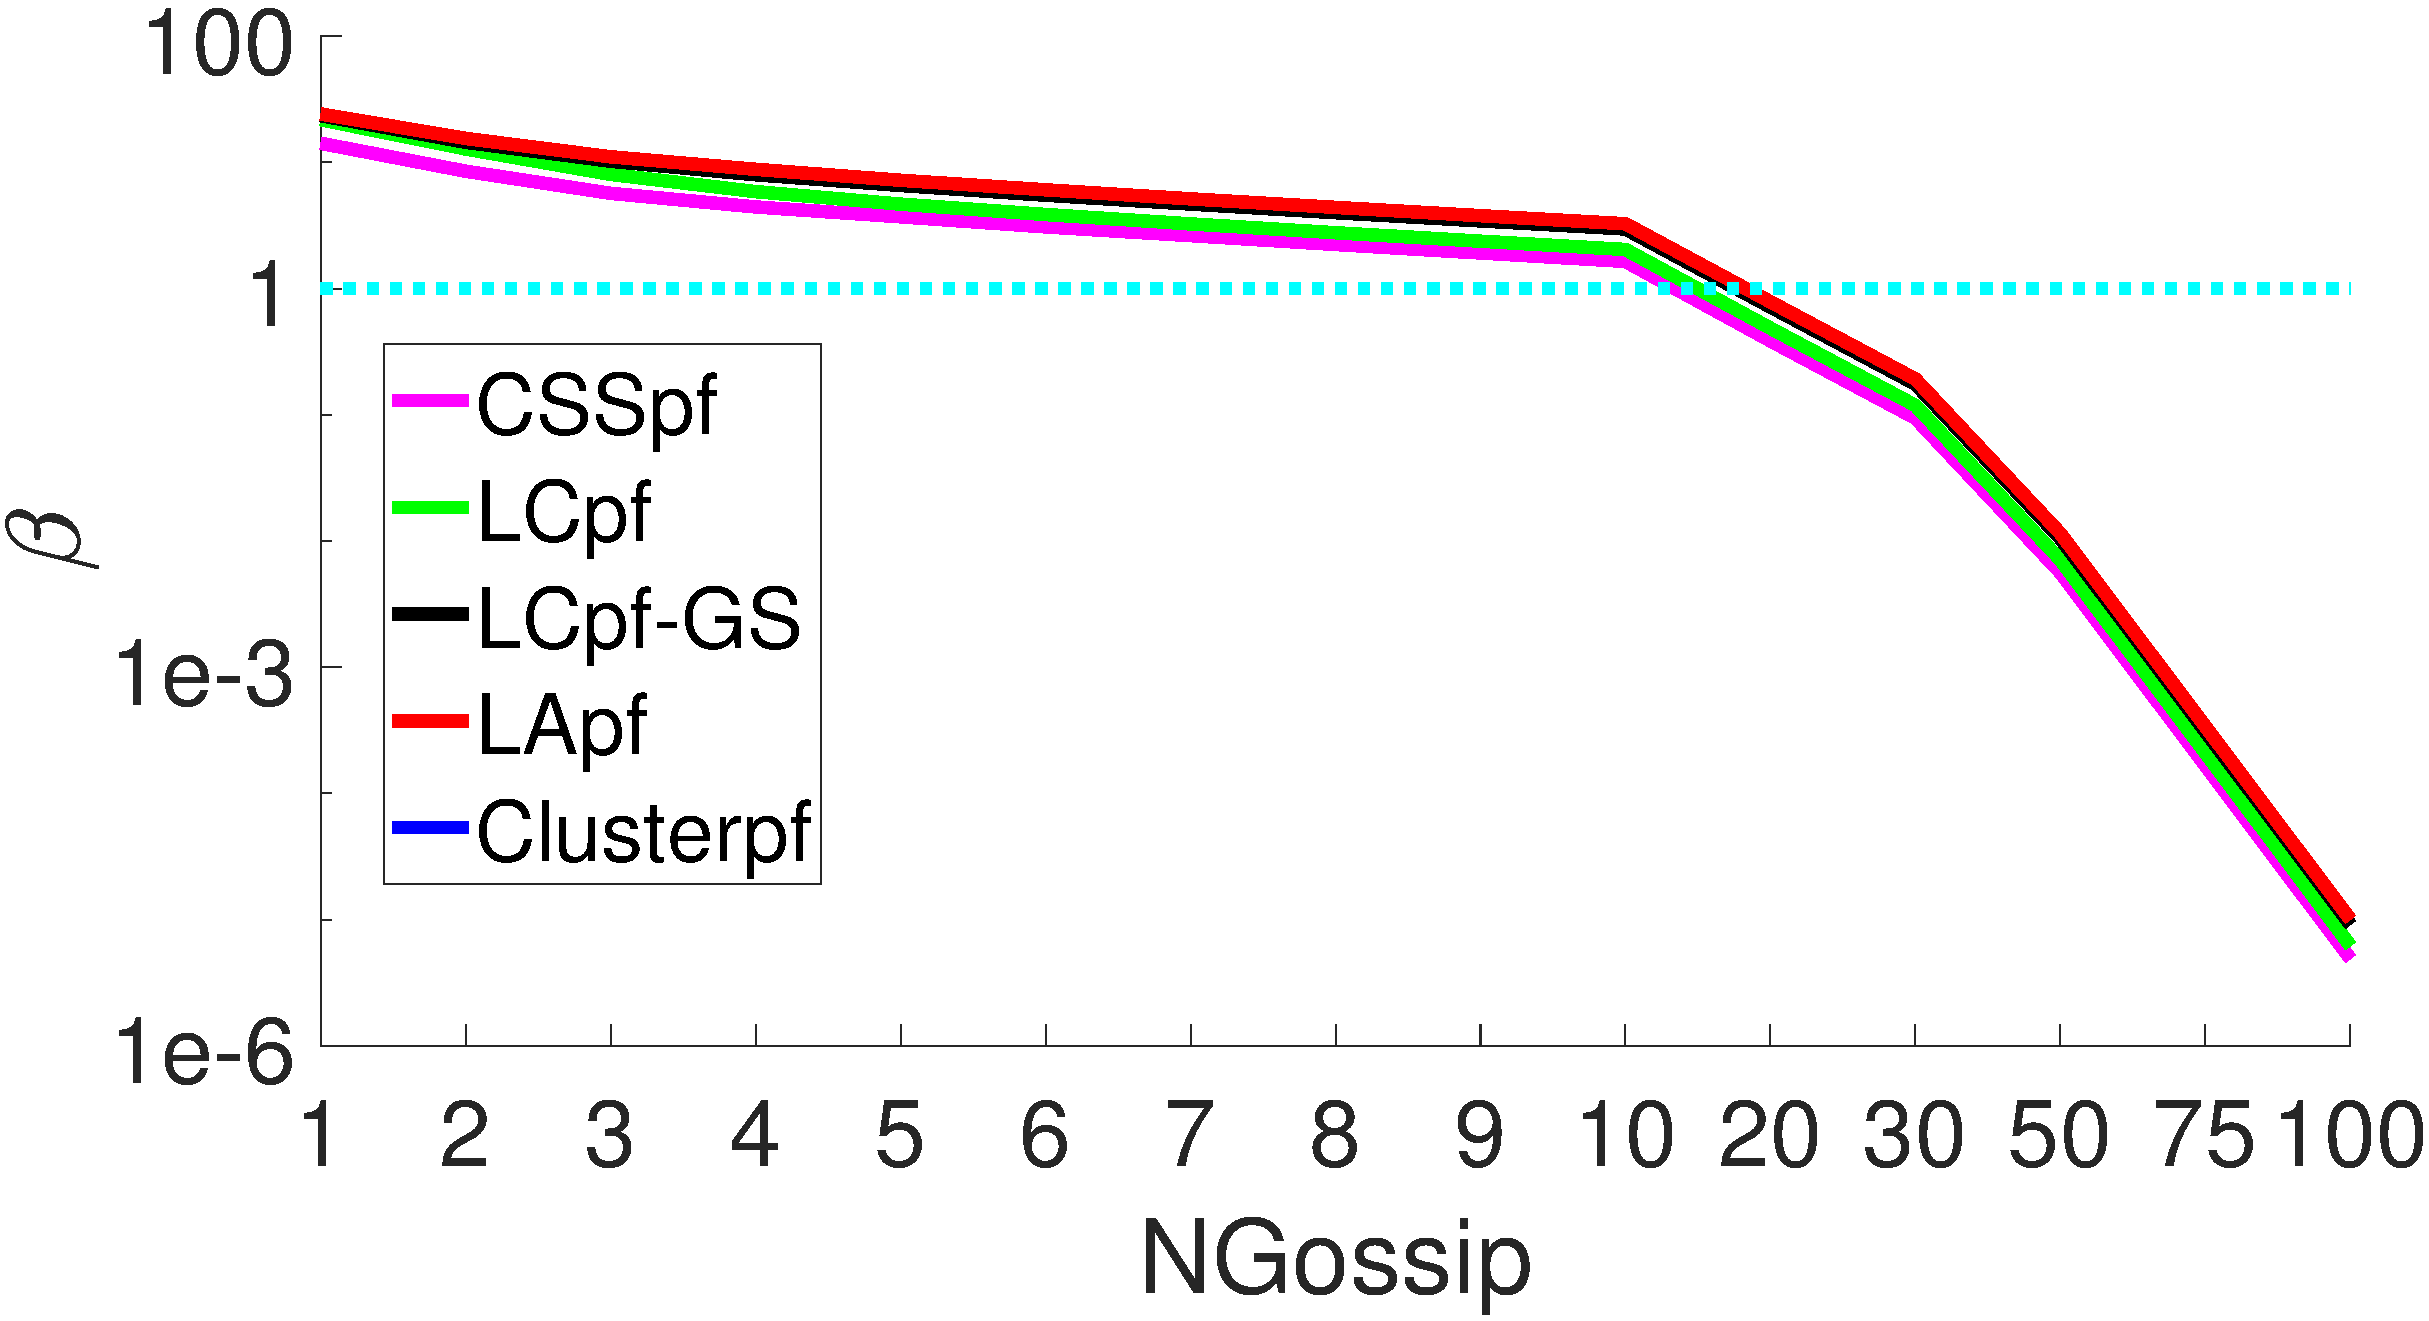
\includegraphics[width=0.49\textwidth]{Figures/beta_track2}}
\end{subfigure}
\begin{subfigure}[Average $||\Psi||_\infty||\alpha||_\infty$ over time]
{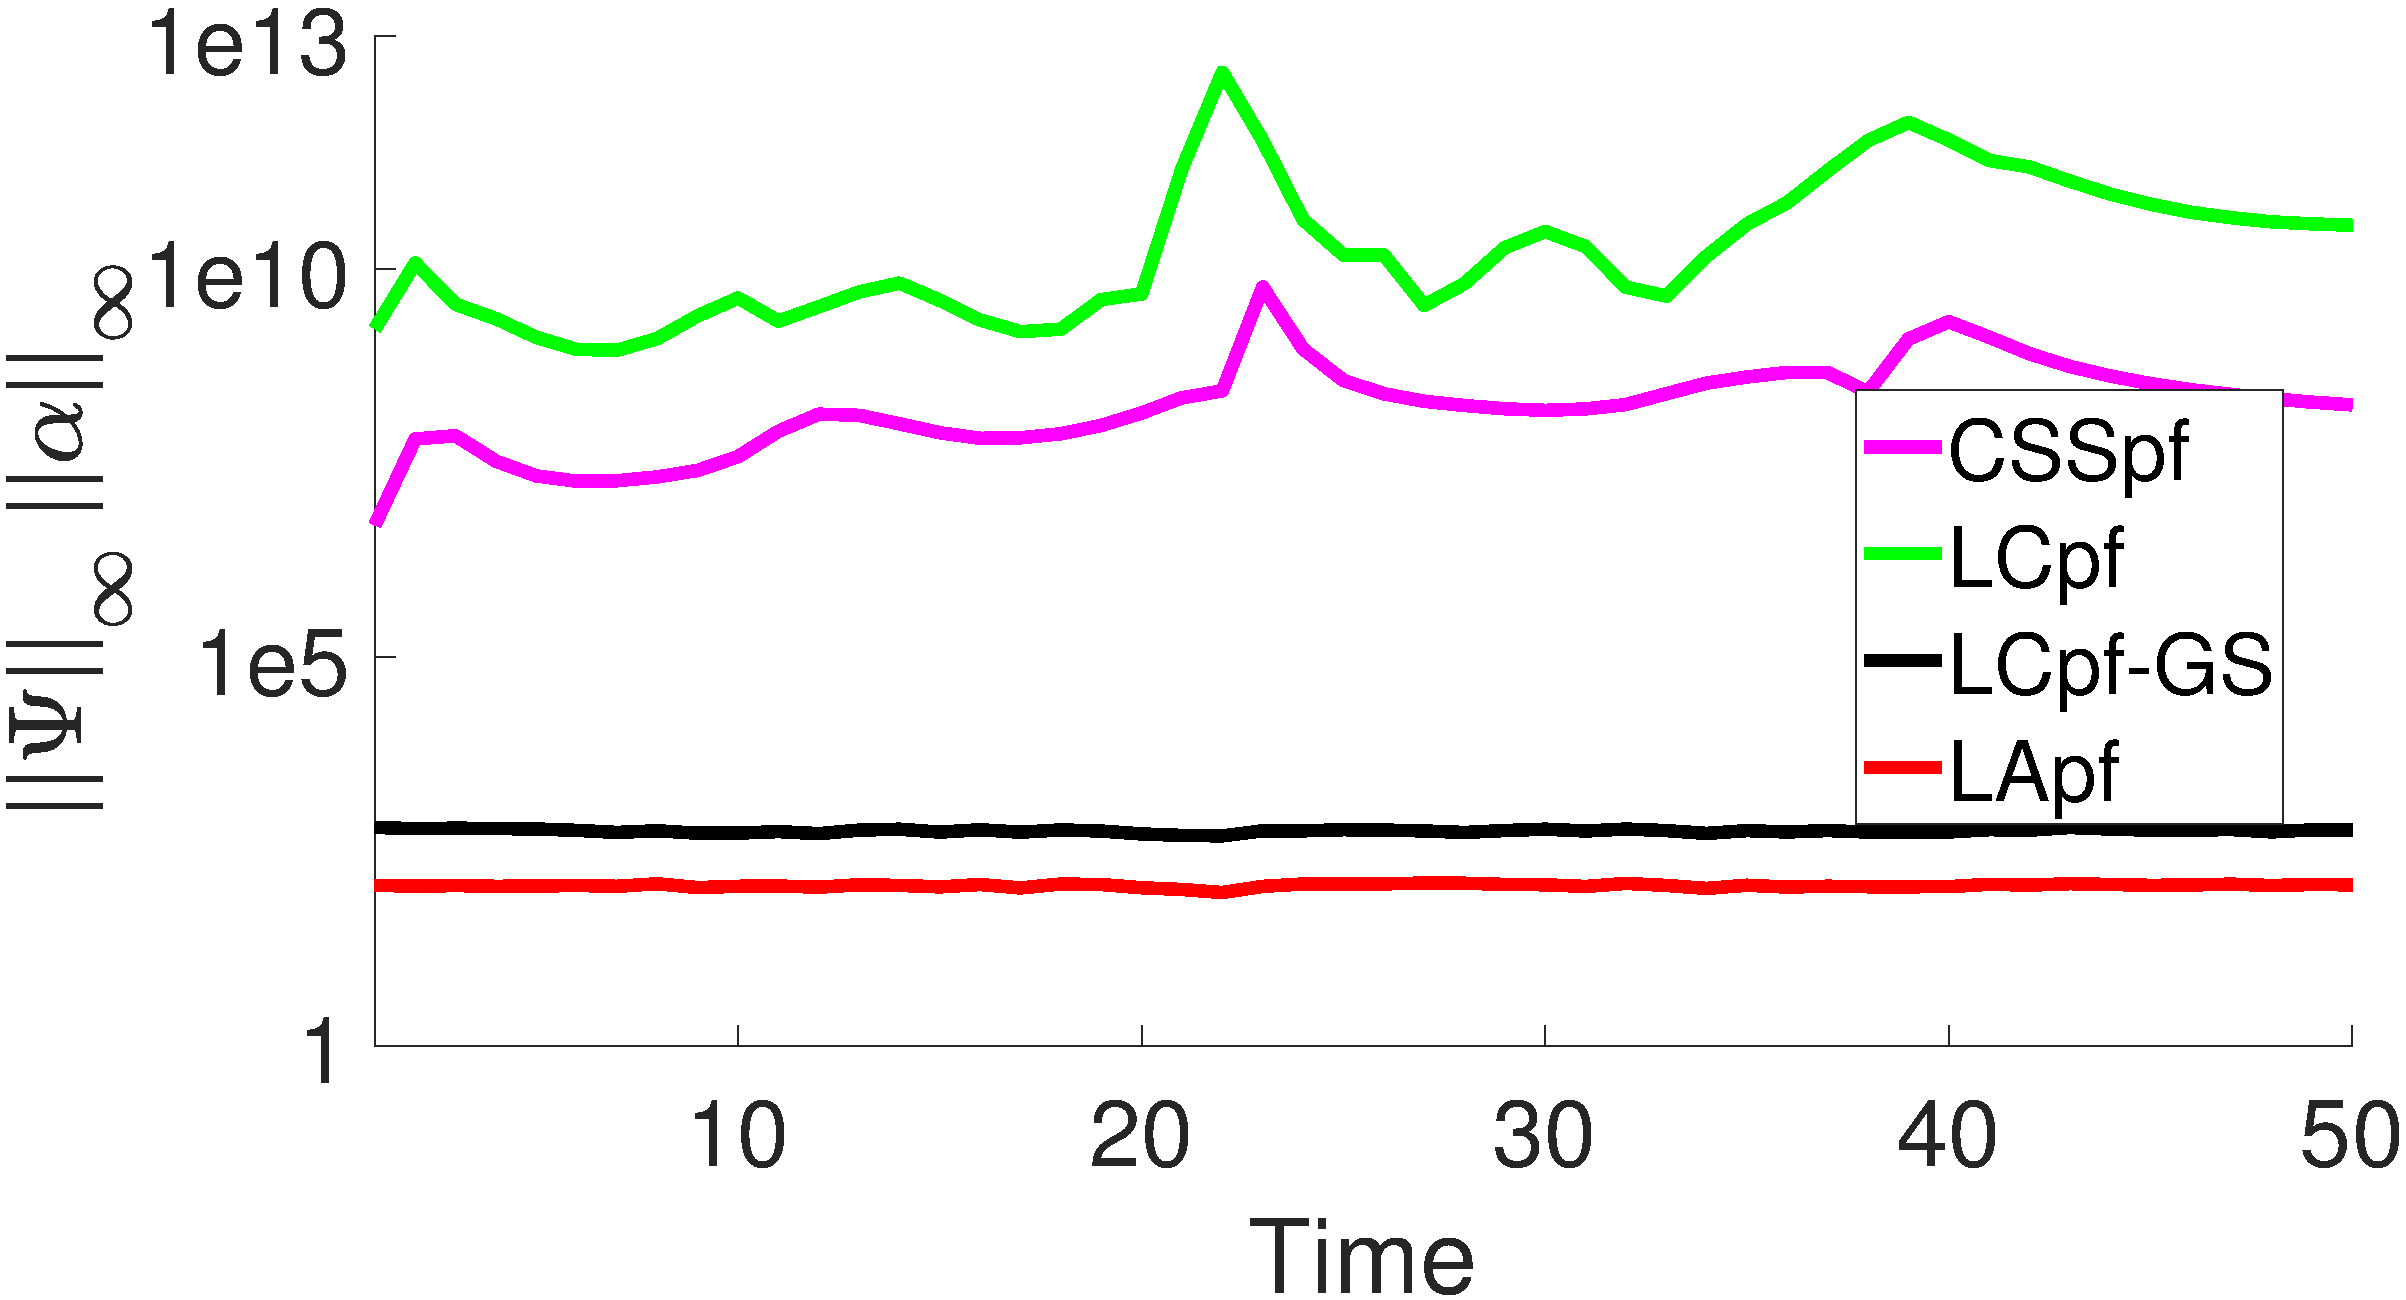
\includegraphics[width=0.49\textwidth]{Figures/Psi_Alpha_track2}}
\end{subfigure}
\begin{subfigure}[Log-likelihood error $\delta$, circles represent true errors and solid lines represent the theoretical higher bound $(1+\delta_m)\delta_{\text{gossip}}+\delta_m$]
{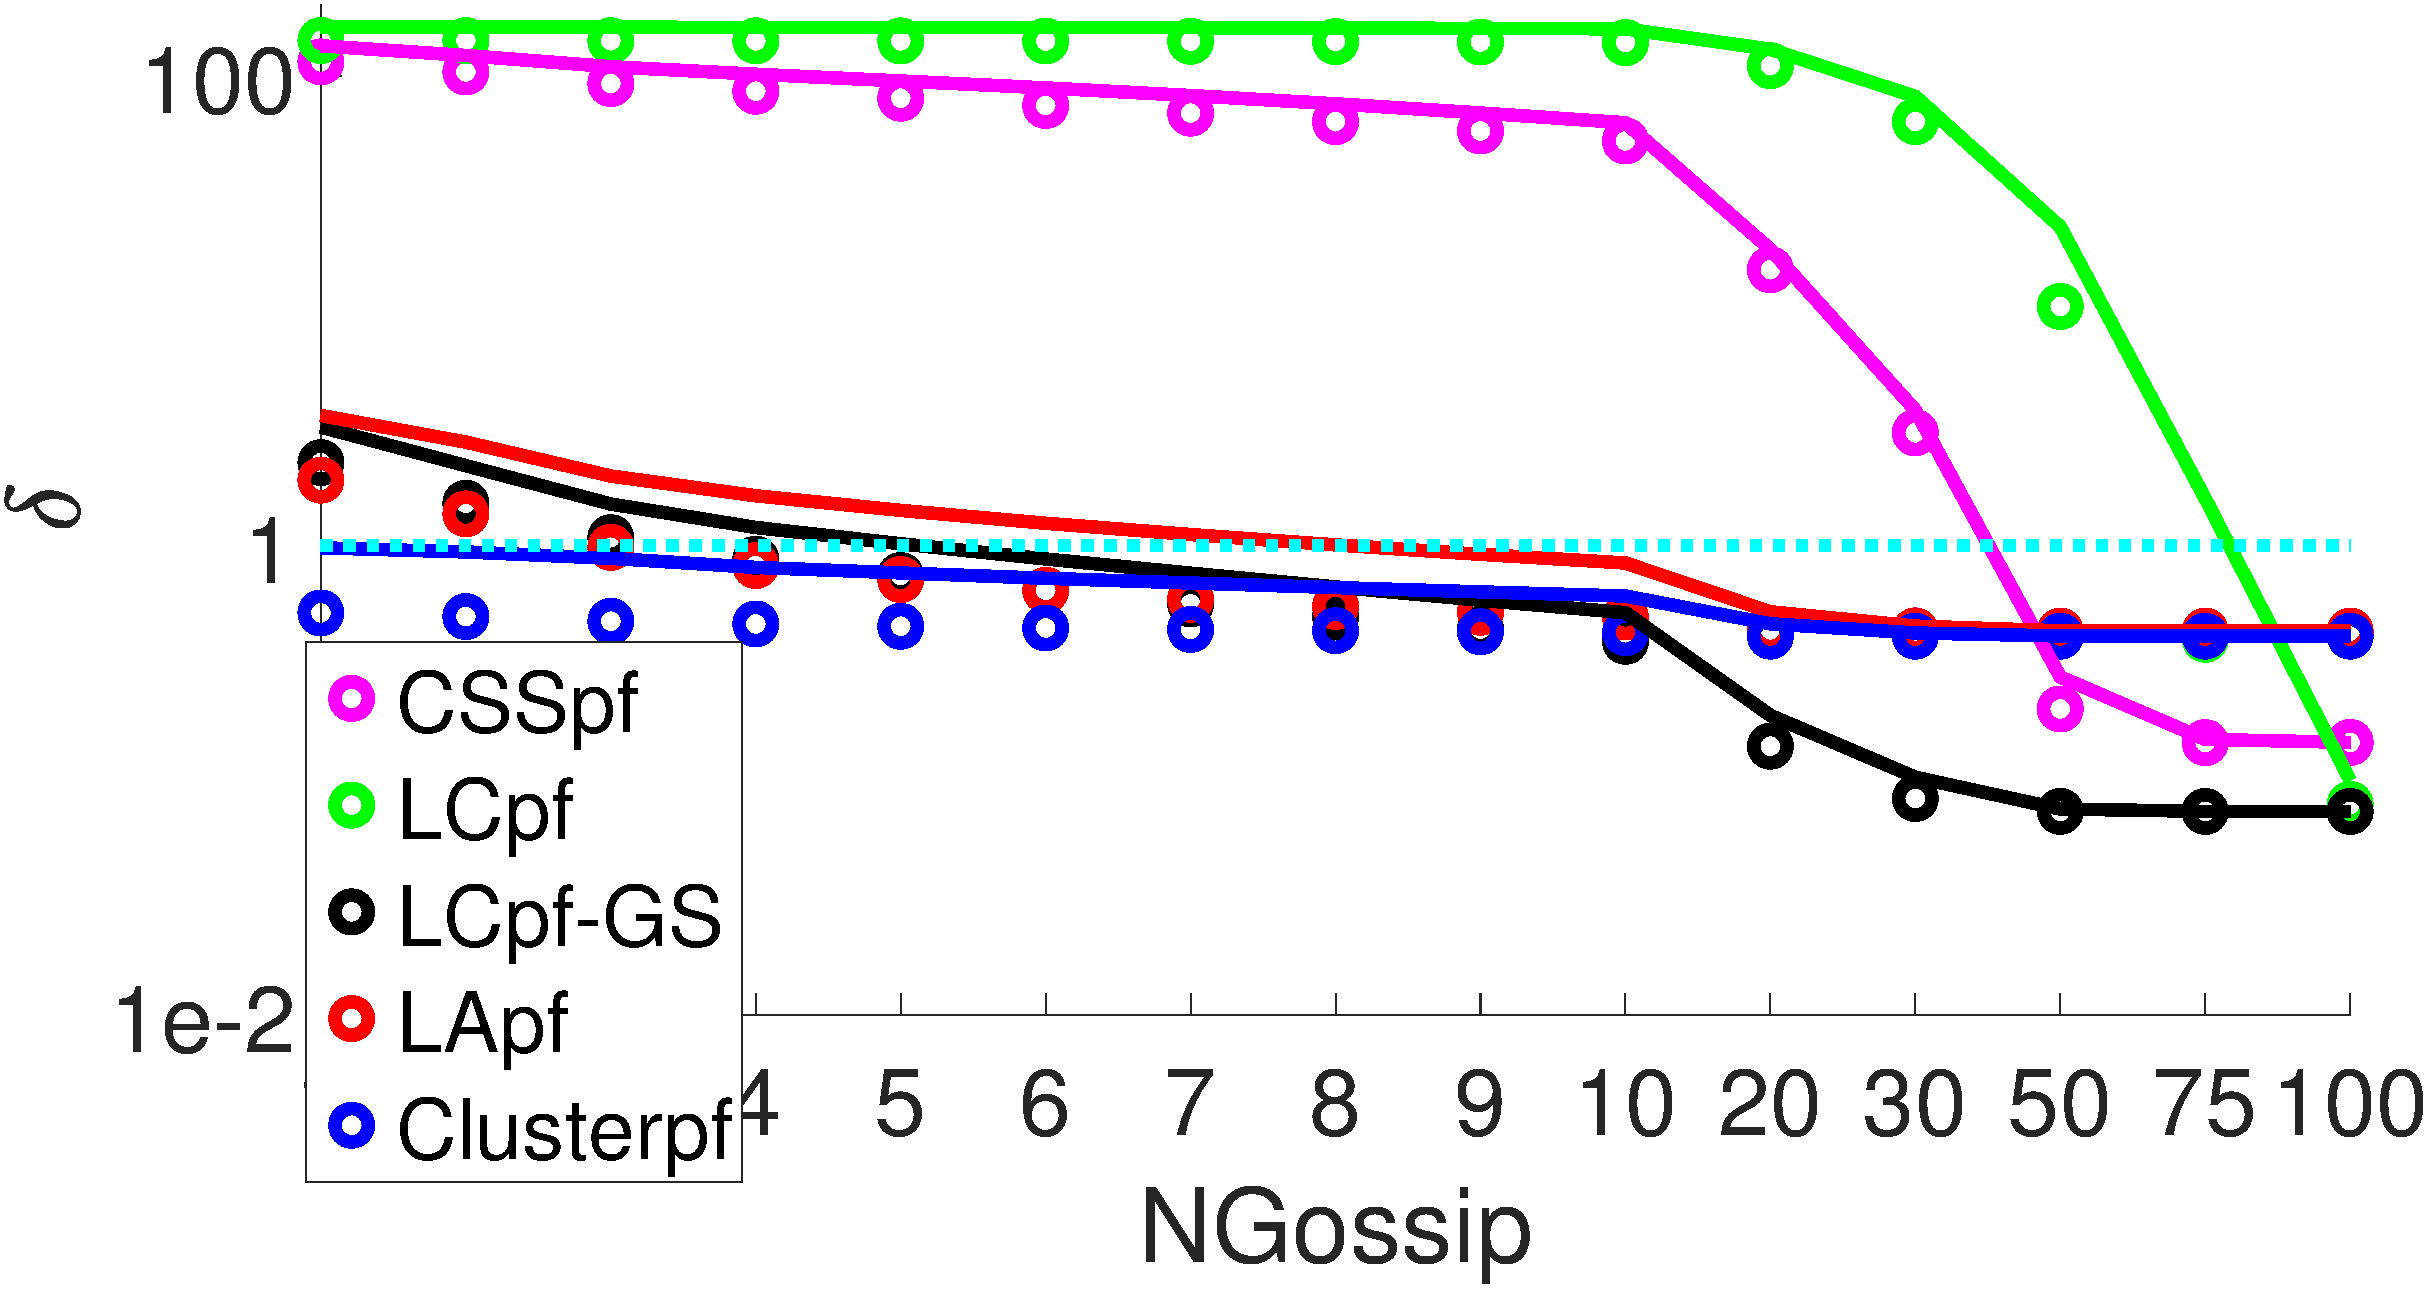
\includegraphics[width=0.49\textwidth]{Figures/delta_bound_track2}}
\end{subfigure}
\begin{subfigure}[Normalized particle weights discrepancy $||w_{\text{true}}-w_{\text{approx}}||_2$]
{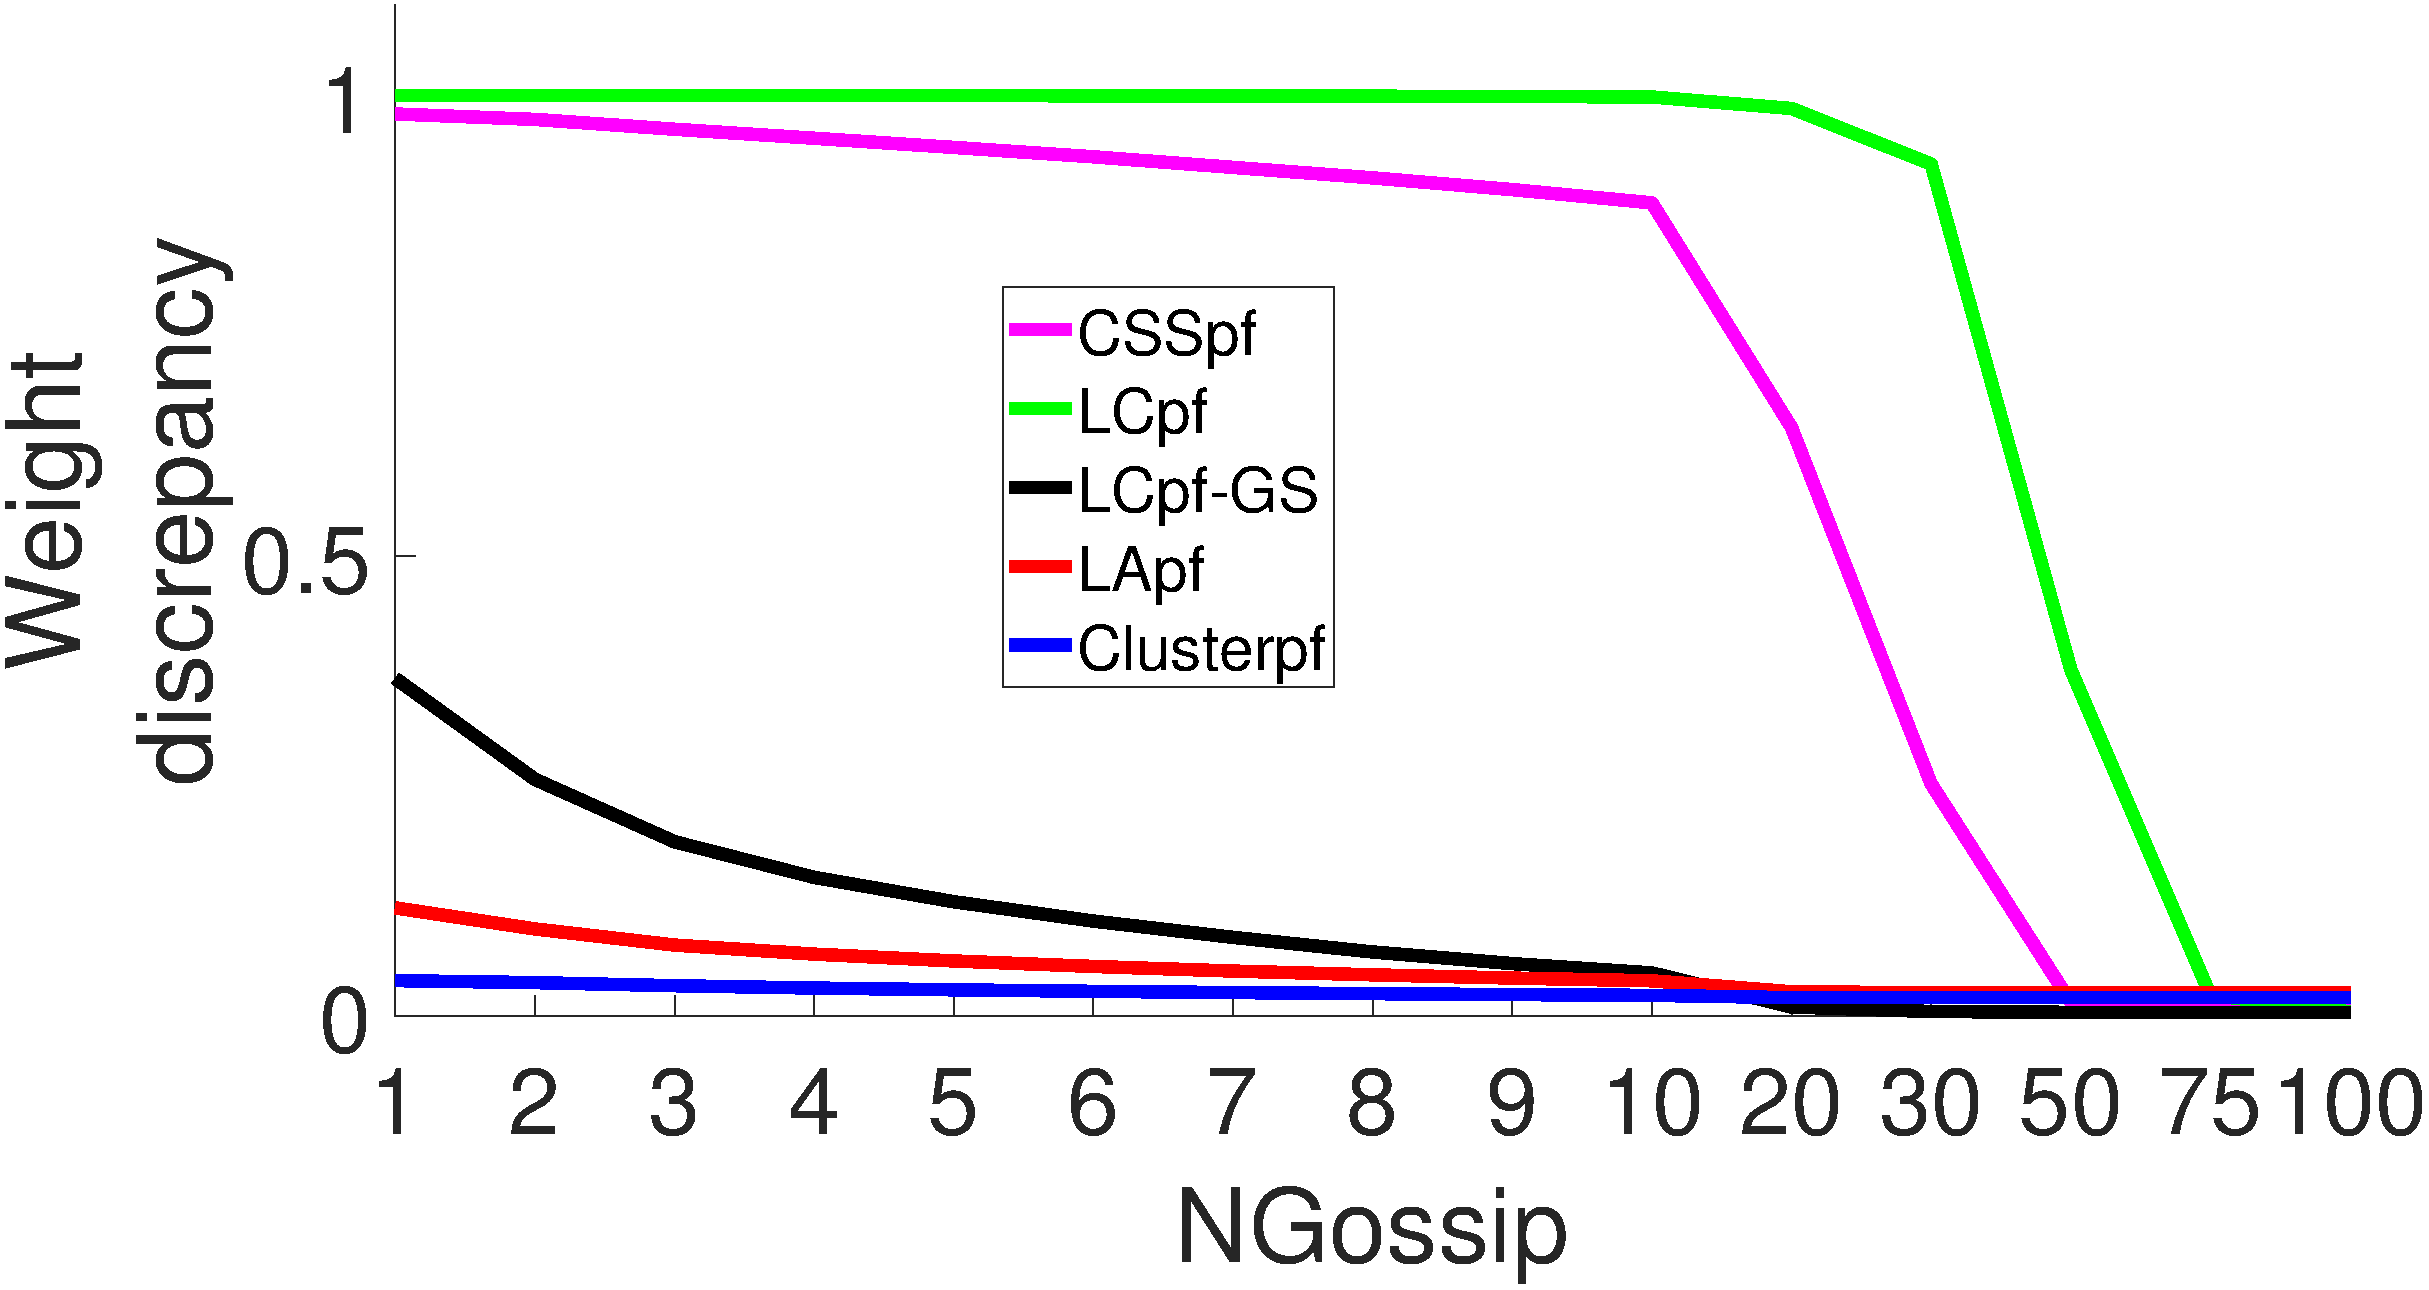
\includegraphics[width=0.49\textwidth]{Figures/Track1_weight_discrepancy}}
\end{subfigure}
\caption{Distributed particle filter error bounds with respect to $NGossip$ and time for track 1. $N=500$, $d=2,m=C=6$.}
\label{fig:detailed_results_track1}
\end{figure}

Fig.~\ref{fig:detailed_results_track1} shows the results for track 1. All data points are averaged over 40 MC trials. Consider first the encoding error $\delta_m$. The LCpf and LCpf-GS have the lowest encoding error followed by CSSpf. The LApf and Clusterpf have the highest encoding error. For all filters, the encoding error spikes for time steps 22 to 23. Otherwise, $\delta_m$ remains below 1. Note that, in our set-up, the actual tracking is done using a centralized BSpf. Therefore, $\gamma_m(X_i)$ and by extension $\delta_m$ remains constant over different values of NGossip.

Consider next the gossiping error. For Clusterpf, the gossiping error is consistently below unity. For LApf and LCpf-GS, the gossiping error drops below 1 for NGossip$>$4; although the gossiping error for both filters is fairly close to 1 even at low NGossip. For CSSpf and LCpf, $\delta_{\text{gossip}}$ falls below 1 only when NGossip exceeds 50 and 75. We also plot the derived upper bounds. While these bounds are quite loose, their trends are consistent with the actual values. 

Fig.~\ref{fig:detailed_results_track1} (c) shows the average value of $\beta = \max_j|\hat{\alpha}_j-\alpha_j|/|\alpha_j|$. The $\beta$ values for all filters are very close. This is not surprising since $\beta$ is independent of the choice of the filters. 

%If we compare the results of Fig.~\ref{fig:detailed_results_track1} (b) and (c), we note that, even though the $\beta$ is similar for all algorithms at all values of NGossip, the gossiping error $\delta_{\text{gossip}}$ can still be quite different across the algorithms. This suggests that additional factors have an important impact on gossiping error. 

Consider Eq.~\eqref{eqn:gossiping_error2}. In the ideal case of $\delta_m=0$ (i.e., perfect reconstruction of log-likelihoods from $m$ coefficients), the denominator of the bound is the same for all algorithms. From the numerator, we have $\delta_{\text{gossip}}\propto \beta||\Psi||_\infty||\alpha||_\infty$ which makes intuitive sense. Therefore, if LApf and LCpf are to achieve the same gossiping error, then we should have
\begin{align}
\frac{\beta^{LC}}{\beta^{LA}} &= \frac{||\Psi^{LA}||_\infty||\alpha^{LA}||_\infty}{||\Psi^{LC}||_\infty||\alpha^{LC}||_\infty}
\label{eqn:gossiping_error_ratio}
\end{align}
Fig.~\ref{fig:detailed_results_track1} (d) shows the average value of $||\Psi||_\infty||\alpha||_\infty$ over time for CSSpf, LCpf, LCpf-GS, and LApf. The LCpf has the largest curve by several order of magnitude followed by CSSpf. Conversely, the LApf has the lowest curve followed by LCpf-GS. This, combined with Eq.~\eqref{eqn:gossiping_error_ratio} suggests that LApf and Clusterpf would indeed require significantly more gossiping iterations to reduce $\beta$ accordingly. For LCpf-GS, the orthogonalization of the encoding matrix reduces the value of $||\Psi||_\infty||\alpha||_\infty$. As a result, LCpf-GS requires less gossiping iterations to achieve robust tracking performance. 

Fig.~\ref{fig:detailed_results_track1} (e) shows the overall error $\delta$. For Clusterpf, $\delta<1$ for all values of NGossip. For LApf and LCpf-GS, $\delta<1$ for $NGossip>4$. For LCpf and CSSpf, the error becomes bounded only when NGossip exceeds 50 and 75 respectively. For all filters, the upper bound $(1+\delta_m)\delta_{\text{gossip}}+\delta_m$ is very close to the true value. As $\delta_m$ is small for all filters, at low NGossip, the gossiping error $\delta_{\text{gossip}}$ becomes the dominating factor and Clusterpf has the lowest $\delta$. At higher NGossip, the encoding error becomes the dominating factor and LCpf-GS has the lowest $\delta$. 

Finally, Fig.~\ref{fig:detailed_results_track1} (f) shows the average discrepancy in normalized particle weights. The curves for CSSpf and LCpf are significantly higher than the other curves until NGossip $>$ 50 and NGossip $>$ 75 as expected. 

%\begin{align}
%\frac{||\gamma_m(x_i)-\hat{\gamma}(x_i)||}{||\gamma_m(x_i)||}&=\frac{||\Psi_i\alpha-\Psi_i\hat{\alpha}||}{||\Psi_i\alpha||} \nonumber \\
%&\geq \frac{||\Psi_i^T\Psi_i\alpha-\Psi_i^T\Psi_i\hat{\alpha}||}{||\Psi_i^T||\cdot ||\Psi_i\alpha||}
%\end{align} 
%where the inequality follows from $||\Psi_i^T\Psi_i \alpha|| \leq ||\Psi_i^T||\cdot ||\Psi_i\alpha||$.

%an upper bound for the gossiping error as follows:
%\begin{align}
%\frac{||\gamma_m(x_i)-\hat{\gamma}(x_i)||}{||\gamma_m(x_i)||}&=\frac{||\Psi_i\alpha-\Psi_i\hat{\alpha}||}{||\Psi_i\alpha||} \\
%&\leq ||\Psi_i^T||\frac{||\Psi_i\alpha-\Psi_i\hat{\alpha}||}{||\Psi_i^T\Psi_i\alpha||} \\
%&\leq ||\Psi_i^T|| \cdot ||\Psi_i||\cdot \frac{||\alpha-\hat{\alpha}||}{||\Psi_i^T\Psi_i\alpha||} 
%\end{align}
%where the first inequality follows from $||\Psi_i^T\Psi_i \alpha|| \leq ||\Psi_i^T||\cdot ||\Psi_i\alpha||$.

%Depending on the encoding matrix $\Psi$, the upper bound can be quite loose. We follow the same approach and derive a lower bound which may be more useful. 

%\begin{align}
%\frac{||\gamma_m(x_i)-\hat{\gamma}(x_i)||}{||\gamma_m(x_i)||}&=\frac{||\Psi_i\alpha-\Psi_i\hat{\alpha}||}{||\Psi_i\alpha||} \nonumber \\
%&\geq \frac{||\Psi_i^T\Psi_i\alpha-\Psi_i^T\Psi_i\hat{\alpha}||}{||\Psi_i^T||\cdot ||\Psi_i\alpha||}
%\end{align}

\section{Conclusion}

\bibliographystyle{IEEEtran}
\bibliography{refs}
\end{document}